%
%  PARA TRABALLOS EN GALLEGO USAR (LINEA 12): \usepackage[galician]{babel}
%  PARA TRABALLOS EN CASTELLANO USAR (LINEA 13): \usepackage[spanish]{babel}
%
% Para los acentos usamos codificacion UTF-8 (LINEA 10): \usepackage[utf8]{inputenc} 
% Si se usase la codificacion es_ES.ISO-8859-1 (LINEA 11): \usepackage[latin1]{inputenc}
% La conversion de acentos se hace con: iconv -f UTF-8 -t ISO-8859-1 filename.tex
%
% Como se incluyen figuras eps hay que compilar con: latex traballo , dvipdf traballo
%

\documentclass[12pt,twoside,a4paper]{book}
%\documentclass[a4paper,10pt]{article}
% pódense engadir todos os packages necesarios
\usepackage[utf8]{inputenc}
%\usepackage[T1]{fontenc}	%Correct accented characters and copy paste them, also not unexpected results with some characters like pipe


%				%es-noquotes]{babel}			si caracteres dan problemas
%				%es-noshorthands]{babel}		si caracteres dan todavia problemas
%				%es-noindentfirst]{babel}		para eliminar sangría
%\usepackage[latin1]{inputenc}
%\usepackage[galician]{babel}
%\usepackage[spanish]{babel}
%\usepackage[spanish, es-tabla,es-noindentfirst]{babel}		%http://www.tex-tipografia.com/spanishopt.html
%\usepackage[spanish, es-tabla]{babel}		%http://www.tex-tipografia.com/spanishopt.html
\usepackage[english]{babel}		%http://www.tex-tipografia.com/spanishopt.html
\addto\captionsenglish{
  \renewcommand{\contentsname}
    {Index} % ToC will show "Index" instead of "Content"
}

%\usepackage[document]{ragged2e}	%centering

\usepackage{graphicx}
\usepackage[dvips]{epsfig}
\usepackage{amssymb}
\usepackage{eurosym}
\usepackage{float}
\usepackage{latexsym}
\usepackage{a4}
\usepackage{hyperref}

%tables
\usepackage{multirow}
\usepackage{multicol}
%\usepackage{changepage}		%margin, eg for tables before tabular \begin{adjustwidth}{-1.4cm}{}
\usepackage{tabularx}

%\usepackage{color}
\usepackage[table,xcdraw,usenames,dvipsnames]{xcolor}


%WBS
%\usepackage{tikz}
%\usetikzlibrary{arrows.meta,shapes,positioning,shadows,trees}
%\tikzset{
    %basic/.style  = {draw, text width=2cm, drop shadow, font=\sffamily, rectangle},
    %root/.style   = {basic, rounded corners=2pt, thin, align=center,
                     %fill=green!30},
    %onode/.style = {basic, thin, align=center, fill=green!60,text width=3cm,},
    %tnode/.style = {basic, thin, align=left, fill=pink!60, text width=6.5em},
    %edge from parent/.style={->, >={latex}, draw=black, edge from parent fork right}
%}
\usepackage{forest}
\usetikzlibrary{arrows.meta,shapes,positioning,shadows,trees}
\tikzset{
    basic/.style  = {draw, text width=2cm, drop shadow, font=\sffamily, rectangle},
    root/.style   = {basic, rounded corners=2pt, thin, align=center,
                     fill=green!30, text width=2cm,},
    onode/.style = {basic, thin, rounded corners=2pt, align=left, fill=green!60,text width=6cm,},
    tnode/.style = {basic, thin, align=left, fill=gray!30, text width=5cm},
    edge from parent/.style={draw=black, edge from parent fork right}
}


\usepackage{pgfgantt}


%%\usepackage{amsmath}		%https://www.sharelatex.com/learn/Aligning_equations_with_amsmath
%%\usepackage{amsfonts}		%Extended set of fonts for use in mathematics
%%\usepackage{afterpage}		%Commands specified in its argument are expanded after the current page is output. EG: \afterpage{\clearpage} and the current page will be filled up with text as usual, but then the \clearpage command will flush out all the floats before the next text page begins

\usepackage{listings}
%	\lstset{breaklines}			%line wrap for listings
%	\newcommand{\lstlistinginput}{\lstinputlisting}		%alias


\usepackage{courier}		%listings better font
\usepackage[sorting=none]{biblatex} %use with \cite{} and \printbibliography[type=online,heading=subbibliography,title={Referencias web}]
	\addbibresource{capitulos/bib.bib}



%%\usepackage{microtype}		%Improves spacing (words and letters) and more stuff. Load after fonts, because is dependent on this font
%%\usepackage{siunitx}		%SI units
%%\usepackage{xspace}			%Decides whether to insert a space to replace one "eaten" by the command decoder
%%\usepackage{todonotes}		%Mark things to do later
%\usepackage{hyperref}		%\hyperref, \url and \href
%%\usepackage[a4paper]{geometry}	%Margins without needing to remember the particular page dimensions commands. Eg [a4paper], [top=1in, bottom=1.25in, left=1.25in, right=1.25in]
%%\usepackage{cleveref}		%LAST \usepackage in the preamble. If anything else modifies the referencing system (like amsmath) it all goes wrong
%
%%\DisableLigatures{encoding = *, family = *}		%https://en.wikibooks.org/wiki/LaTeX/Text_Formatting#Ligatures
%%\def\spanishoperators{}		%stuff like sin traduced to sen, max to máx, etc



\newcommand\realnumberstyle[1]{}

\makeatletter
\newcommand{\zebra}[3]{%
    {\realnumberstyle{#3}}%
    \begingroup
    \lst@basicstyle
    \ifodd\value{lstnumber}%
        \color{#1}%
    \else
        \color{#2}%
    \fi
        \rlap{\hspace*{\lst@numbersep}%
        \color@block{\linewidth}{\ht\strutbox}{\dp\strutbox}%
        }%
    \endgroup
}
\makeatother

%%%%%%%%%%%%%%%%%%%%%%%%%		MORE	ALIASES		%%%%%%%%%%%%%%%%%%%%%%%%%

\newcommand{\lineh}{\rule{\textwidth}{1pt}\hfill\break}
\newcommand{\linej}{\hfill\break}

\newcommand{\IncrementoSiete}{VirusTotal integration}
\newcommand{\IncrementoSeis}{Additional detection for GNU/Linux}
\newcommand{\IncrementoCinco}{Explore solutions in problems with GPDR}
\newcommand{\IncrementoCuatro}{Adapt Wazuh configuration to typical requirements from enterprises}
\newcommand{\IncrementoTres}{Detection/action against ransomware}
\newcommand{\IncrementoDos}{Use of data from Sysmon}
\newcommand{\IncrementoUno}{Common attacks in Windows Server}



%%%%%%%%%%%%%%%%%%%%%%%%%		END BASIC CONF		%%%%%%%%%%%%%%%%%%%%%%%%%



%\definecolor{mygreen}{rgb}{0,0.6,0}
%\definecolor{mygray}{rgb}{0.5,0.5,0.5}


%\renewcommand{\thesubsection}{\thesection.\alph{subsection}}		%change subsection style to letters



%https://en.wikibooks.org/wiki/LaTeX/Source_Code_Listings

%\lstdefinestyle{C} {
%	language=C,		%for syntax highlighting
%	basicstyle=\footnotesize\ttfamily,
%	frame=tb,
%	tabsize=4,
%	columns=fixed,
%	showstringspaces=false,
%	showtabs=false,
%	keepspaces,
	%commentstyle=\color{gray},
	%stringstyle=\color{brown},
	%keywordstyle=\color{blue},
	%directivestyle=\color{gray},			%preprocessor color
	%emph={int,char,double,float,unsigned},
	%emphstyle=\color{green},
%}
%\lstset{ language=C }	%		\begin{lstlisting}[style=C]		\lstinputlisting[style=C]{main.c}



%\lstdefinestyle{sql} {
%	language=sql,		%for syntax highlighting
%	basicstyle=\footnotesize\ttfamily,
%	frame=tb,
%	tabsize=4,
%	columns=fixed,
%	showstringspaces=false,
%	showtabs=false,
%	keepspaces,
%	commentstyle=\color{red},
%	stringstyle=\color{orange},		%needs xcolor
%	keywordstyle=\color{blue}
%}
%\lstset{ language=sql }		\begin{lstlisting}		\lstinputlisting[style=sql]{file.sql}




%\lstdefinestyle{sh} {
	%language=sh,		%for syntax highlighting
	%basicstyle=\footnotesize\ttfamily,
	%frame=tb,
	%tabsize=4,
	%columns=fixed,
	%showstringspaces=false,
	%showtabs=false,
	%keepspaces,
	%commentstyle=\color{gray},
	%stringstyle=\color{brown},
	%keywordstyle=\color{blue},
	%directivestyle=\color{gray},			%shebang color
	%emph={local, export },
	%emphstyle=\color{green},
%}
%\lstset{ language=sh }			%\begin{lstlisting}		\lstinputlisting[style=sh]{script.sh}


%\lstdefinestyle{python} {
	%language=python,		%for syntax highlighting
	%basicstyle=\footnotesize\ttfamily,
	%frame=tb,
	%tabsize=4,
	%columns=fixed,
	%showstringspaces=false,
	%showtabs=false,
	%keepspaces,
	%commentstyle=\color{gray},
	%stringstyle=\color{brown},
	%keywordstyle=\color{blue},
	%directivestyle=\color{gray},			%shebang color
	%emphstyle=\color{green},
%}
%\lstset{ language=python }			%\begin{lstlisting}		\lstinputlisting[style=python]{script.py}



%\lstdefinestyle{file} {
	%basicstyle=\footnotesize\ttfamily,
	%frame=tblr,
	%tabsize=4,
	%columns=fixed,
	%showstringspaces=false,
	%showtabs=false,
	%keepspaces,
	%title=\lstname
%}


\lstdefinestyle{xml} {
	language=XML,		%for syntax highlighting
	basicstyle=\footnotesize\ttfamily,
	numbers=left,
	numberstyle=\tiny\zebra{green!10}{white},
	frame=tb,
	postbreak=\mbox{\textcolor{red}{$\hookrightarrow$}\space},
	tabsize=4,
	columns=fixed,
	showstringspaces=false,
	showtabs=false,
	keepspaces,
	commentstyle=\color{red},
	stringstyle=\color{orange},		%needs xcolor
	keywordstyle=\color{blue}
}

%\lstset{		%basicstyle=\small\sffamily,
	%basicstyle=\footnotesize\ttfamily,
	%numbers=left,
	%numberstyle=\tiny\zebra{green!10}{white},
	%frame=tb,
	%tabsize=4,
	%columns=fixed,
	%showstringspaces=false,
	%showtabs=false,
	%keepspaces,
	%commentstyle=\color{red},
	%stringstyle=\color{orange},
	%extendedchars=true,
	%literate={á}{{\'a}}1
	%{é}{{\'e}}1
	%%{í}{{\'{\i}}}1
	%{í}{{\'i}}1
	%{ó}{{\'o}}1
	%{ú}{{\'u}}1
	%{Á}{{\'A}}1
	%{É}{{\'E}}1
	%{Í}{{\'I}}1
	%{Ó}{{\'O}}1
	%{Ú}{{\'U}}1
	%%{ü}{{\"u}}1
	%%{Ü}{{\"U}}1
	%{ñ}{{\~n}}1
	%{Ñ}{{\~N}}1
	%{¿}{{?``}}1
	%{¡}{{!``}}1,
	%keywordstyle=\color{blue}
%}




%atm general file listing with
%\lstinputlisting[style=file]{}


%%%%%%%%%%%%%%%%%%%%%%%%%		END CURRENT DOCUMENT CONF		%%%%%%%%%%%%%%%%%%%%%%%%%








\begin{document}

\pagestyle{empty}
\begin{center}
{\bf\Large UNIVERSITY OF SANTIAGO DE COMPOSTELA}

\vspace{0.5cm}

\includegraphics[width=5cm]{figuras/logo_usc.eps}

\vspace{0.5cm}
{\bf\large ESCOLA TÉCNICA SUPERIOR DE ENXEÑARÍA}

\vspace{2cm}
{\bf\LARGE Improvements in IDS: adding functionality to Wazuh}

%\vspace{0.5cm}
%{\bf\LARGE Subtítulo do Traballo de Fin de Grao}
\end{center}

\vspace{2cm}
\hspace{4cm}\begin{tabular}{l}
{\it\Large Autor:} \\
{\bf\Large Andrés Santiago Gómez Vidal} \\
~ \\
{\it\Large Directores:} \\
{\bf\Large Purificación Cariñena Amigo} \\
{\bf\Large Andrés Tarascó Acuña} \\
\end{tabular}

\vspace{2cm}
\begin{center}
{\bf\Large Computer Engineering Degree}

\vspace{0.5cm}
{\bf\large July 2019}

\vspace{0.5cm}
Final degree project presented at the Escola Técnica Superior de Enxeñaría of the University of Santiago de Compostela to obtain the Degree in Computer Engineering
\end{center}


\cleardoublepage
\pagestyle{plain}
\pagenumbering{roman}

\includegraphics[width=4cm]{figuras/logo_usc.eps}

\vspace{1cm}
{\bf Ms. Purificación Cariñena Amigo}, Professor Computing Science and Artificial Intelligence at the University of Santiago de Compostela and {\bf Mr. Andrés Tarascó Acuña}, Managing Director at Tarlogic Security S.L.

\vspace{1cm}
STATE:

\vspace{1cm}
That the present report entitled \textit{Improvements in IDS: adding functionality to Wazuh} written by \textbf{Andrés Santiago Gómez Vidal} in order to obtain the ECTS corresponding to the final degree project of the Computer Engineering degree was conducted under our direction in the department of Computer Science and Artificial Intelligence of the University of Santiago de Compostela.

\vspace{1cm}
For the purpose to be duly recorded, this document was signed in Santiago de Compostela on July 24, 2019:

\vspace{2cm}
%cambiado el tamaño de letra para que quepa mi nombre entero
\footnotesize
\begin{tabular}{lll}
The director, & The codirector, & The student, \\
~ \\
~ \\
~ \\
~ \\
~ \\
~ \\
~ \\
(Purificación Cariñena Amigo) & (Andrés Tarascó Acuña) & (Andrés Santiago Gómez Vidal)
\end{tabular}
\normalsize
 % paxina de certificación (optativa)
\cleardoublepage
%\pagestyle{plain}
%\chapter*{Agradecementos}
%Se se quere pór algún agradecemento, este vai aquí.

%TODO
 % paxina de agradecementos (optativa) 
\cleardoublepage
%\pagestyle{plain}
%\chapter*{Resumo}
%Se se quere pór resumo, este vai aquí.

%TODO
 % páxina de resumo (optativa) 

\cleardoublepage
\pagestyle{plain}
\tableofcontents
\listoffigures
\listoftables

% Agora incluimos os capítulos. Cambiamos a numeración e as cabeceiras
\cleardoublepage
\pagenumbering{arabic}
\setcounter{page}{1}
\pagestyle{headings}
%Introdución: composta por Obxectivos Xerais, Relación da Documentación que conforma a Memoria, Descrición do Sistema, Información Adicional de Interese (métodos, técnicas ou arquitecturas utilizadas, xustificación da súa elección, etc.).

This project was made in collaboration with the cybersecurity company Tarlogic SL, even though I am not a member of Tarlogic and have never worked with them in the past.
Due to my lack of professional experience in cybersecurity and the need to research in this project, the scope and planning of the work had to be rescheduled.
Furthermore in this project there are no absolute constraints or objectives, as it was suggested as a case between investigation (with some coding) and cybersecurity auditing, so the scope can be reduced if the time remaining is too short.

\section{Motivation}

Cybersecurity nowadays is very complex: there are many sub-fields and expert tools and it could be argued that is impossible to guarantee that any system is totally safe.
In this project we put ourselves in the shoes of a system administrator for an enterprise, that wants to improve the security by detecting intrusions in the servers he works on. This is key to decide which technologies and tools we choose in this project.
\linej
\linej
Cybersecurity measures can be applied in multiple layers of the system, each with different tools, objectives, advantages and costs.
In general the security of a system can be divided into the next parts:
\begin{enumerate}
	\item \textbf{Firewall}: Control the inbound/outbound connections, on the \textbf{network layer}. In our scenario its objective is to reduce the amount of inbound connections, reducing the chance of intrusion.
	\item \textbf{IPS}: Intrusion Prevention System to minimize the chance of intrusions, on the \textbf{network and host layers}. Provides active protection by actions.
	\item \textbf{IDS}: Intrusion Detection System to mitigate the damage of intrusions, on the \textbf{network and host layers}. Provides passive protection by alerts.
\end{enumerate}

\linej
The next table shows a \textbf{simplified} flow on how the information is processed by the security layers and methods.
For example an IDS can monitor the network connections, scanning the whole packet (header and payload) and filing a report if needed, but has worse performance than a firewall because they only scan the header of the packet and just opt to reject them\cite{firewall-ipds-ids_comparison}.
IDS fall into the SIEM category: software that manages information and events in real-time.

\begin{table}[H]
	\centering
	\caption{Simplification of the data flow}
\linej
	\begin{tabular}{|c|c|c|c|}
	\hline
		\textbf{Layer} & \textbf{Network} & \multicolumn{2}{c|}{\textbf{Network and Host}}\\ \hline
		\textbf{Method} & Firewall & IPS & IDS\\ \hline
		\textbf{Measures} & Prevent & Prevent & Mitigate\\ \hline
	\end{tabular}
\end{table}
$\xrightarrow{\makebox[\textwidth]{Direction of the data flow}}$

\linej
\linej
An IDS that focus on network monitoring is a NIDS.
They have become widely used over the past two decades because of the impressive capability to provide a granular view of what is happening on the network.
\linej
Attackers have grown used to NIDSs and have found ways to evade them, like\cite{libro_ossec}:
\begin{enumerate}
	\item Avoid using known patterns in their connections.
	\item Use encrypted connections.
	\item Send the data in pieces accross the network. This does not work against NIDSs that can reassemble them, at a greater computing cost. %session splicing and framentation attacks
	\item Denial of Service attacks: too much traffic overloads the NIDS, blinding it.
\end{enumerate}
\linej
We understand that NIDSs are useful in many situations, and there are many cases in this project where they could be used to complement an HIDS.
An HIDS can inspect the full stream of communications, making useless the techniques 2 and 3 in the previous example for evading NIDSs.
\linej
We focus on HIDS because we are more interested about detection at host level, rather than network.
Also IDS is less explored than IPS or firewalls and due to the advance in gathering and processing of data in the last years IDS has become much more viable and reliable.

\linej
\linej
IDSs are different from antivirus or antimalware because the first are systems \textbf{specialized} in detection and the latter usually focus on prevention, however prevention and detection are often meshed together because both are deeply related. There are some cases where a system specialized in detection offers some kind of mitigation functionality or one specialized in prevention offers some kind of detection functionality.

\linej
\linej
It is important to note that in cybersecurity the trend is for the attack to be created first and later some kind of measures, not necessarily by the same teams as they usually are specialized in each role. This means that defensive security that requires manual intervention often lags behind.
\linej
Nowadays there are lots of different attacks, so many that their detection could be almost impossible one by one, but most of them can be detected because they share patterns. If we can determine the patterns of an attack and code a way to detect them we can detect the threat. Some times is easier to detect the attack and take measures after the intrusion has taken place.
\linej
\linej
IDSs work by analysing the key information available (programs, logs, network information, etc) to determine if there has been an intrusion in the system. The details of the process vary with each IDS but in general they work like an expert system:
\begin{itemize}
	\item The source of the data is the system.
	\item The alerts are set by certain rules when they match.
	\item Rules do not need to throw an alert and there can be dependencies, allowing a stateful approach and complex analysis without false positives (the main annoyance of IDSs).
\end{itemize}

\linej
There are two types of IDS, based on the detection mechanism:
\begin{itemize}
	\item Signature based: The IDS looks for specific data (signature), for example a string. This is often an efficient solution to known attacks, but is fundamentally useless against unknown attacks (attacks without a signature in the IDS database).
	\item Behaviour analysis: After a training period the IDS can detect when an event is rare (by probability) and correlate these suspicious occurrences to an intrusion.
\end{itemize}
In our case we take interest in the signature approach because is much more used and behavior analysis is more fit for network than host.

\linej
\linej
OSSEC is an HIDS (Host-based IDS) solution with detection based on rules and decoders. Both rules and decoders can be defined with numerous options and support dependencies and regular expressions.
\begin{itemize}
	\item The decoders format the data for the rules.
	\item There is a threat if the conditions of the rule are met.
\end{itemize}
\linej
\textbf{OSSEC} stands for \textbf{O}pen \textbf{S}ource HIDS \textbf{SEC}urity and is interesting for this project because\cite{ossec}\cite{wazuh_additional_functionality}:
\begin{itemize}
	\item \textbf{Widely Used}: OSSEC is a growing project, used by many different entities (ISPs, universities, governments, large corporate data centers) as their main HIDS solution. In addition to being deployed as an HIDS, it is commonly used strictly as a log analysis tool, monitoring and analyzing firewalls, IDSs, web servers and authentication logs.
	\item \textbf{Scalable}: Because it is an HIDS and it uses \textbf{agents}. Each monitored host can either install the agent or use an agentless agent\cite{agentless}\cite{ossec_agent}. Agentless agents are processes initiated from the OSSEC manager, which gather information from remote systems, and use any RPC method (e.g. ssh, snmp rdp, wmi).
	\item \textbf{Multi-platform}: GNU/Linux, Windows, Mac OS and Solaris. This is important because most professional services are on GNU/Linux or Windows, but it is important to note that rules can only work in one operating system.
	\item \textbf{Free}: OSSEC is a free software and will remain so in the future; you can redistribute it and/or modify it under the terms of the GNU General Public License (version 2) as published by the FSF -- Free Software Foundation.
	\item \textbf{Open source}: The code is open, so you can read, contribute and debug it all you want.
	\item \textbf{Rootkits detection}: This type of malware usually replaces or changes existing operating system components in order to alter the behavior of the system. Rootkits can hide other processes, files or network connections like itself.
	\item \textbf{File integrity monitoring}: To detect access or changes to sensitive data.
\end{itemize}
\linej
There are lots of alternatives to OSSEC for the scenario of a system administrator that wants to reinforce the security of the systems he is responsible for. There are free of charge and paid solutions. Not all are pure IDSs and often they specialize in a field. For example the next table shows a comparison of the most important ICSs (Industrial Control Systems):
\begin{figure}[H]
  \centering
	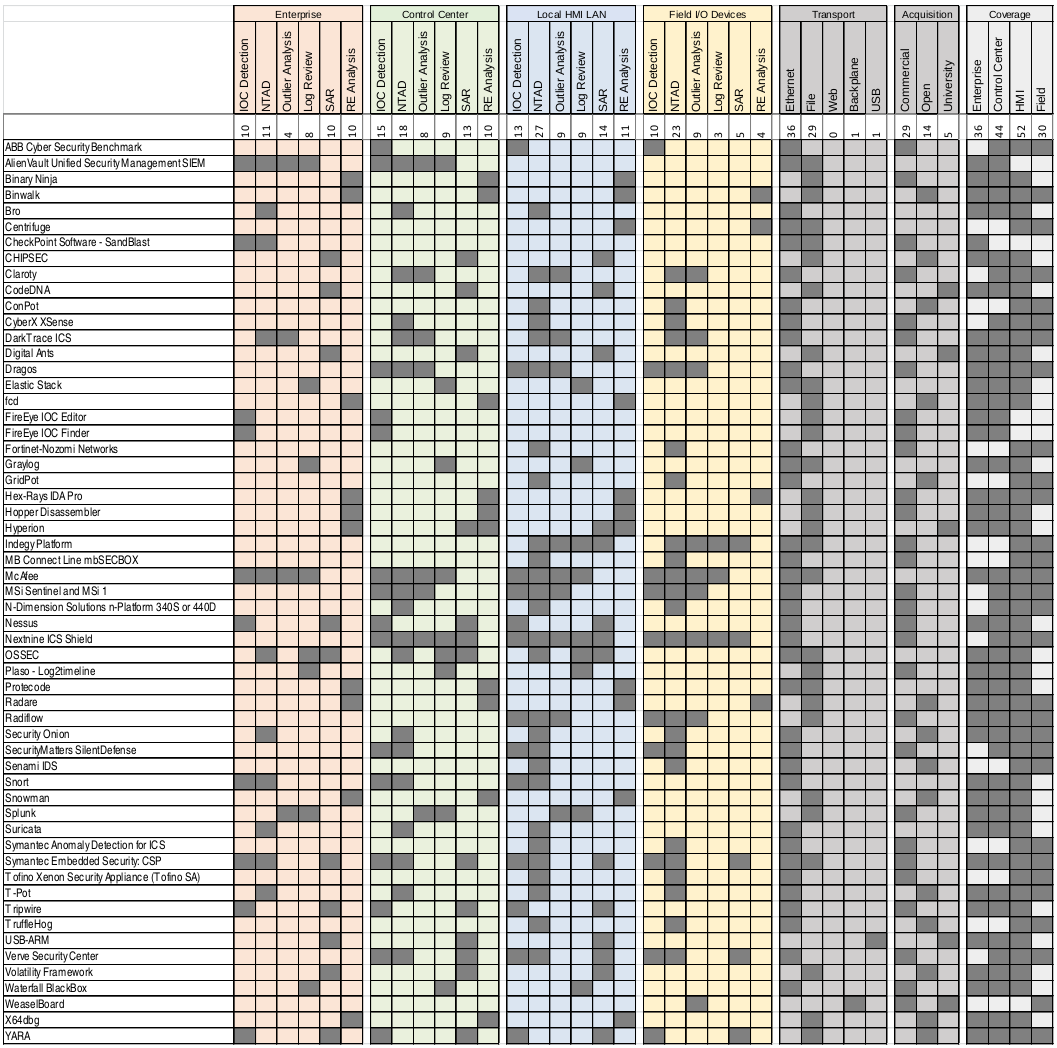
\includegraphics[width=\textwidth]{figuras/comparison_ics.png}
	\caption{Comparison by attributes of the most important ICSs\cite{comparison_ics}}
\end{figure}

\linej
\linej
One of the problems of a comparison in a table like this is that it fails to show how much a tool excels or lacks in the features it shares with others, how easy it is to use and other factors that can decide the right tool. The most relevant alternative technologies to OSSEC for this project are\cite{comparison_tools}:
\begin{itemize}
	\item Sagan: An open source HIDS, but only supports *nix operating systems (Linux, FreeBSD, OpenBSD, etc) and it lacks in features compared to OSSEC.
	\item YARA: Is not an IDS or IPS, it is just a tool that does pattern/string/signature matching, but it excels at it in performance, results and easiness to write the rules. It can be used to scan the \textbf{memory} for known patterns. YARA is being used widely in cybersecurity, for example by Avast, Kaspersky Lab, VirusTotal and McAfee Advanced Threat Defense\cite{who_is_using_yara}. We could build a system to use YARA to scan files but always combined with at least another tool, but we prefer to stick to a tested IDS.
\end{itemize}
\linej
Due to their popularity is worth mentioning the next tools, even though they are only for network:
\begin{itemize}
	\item Bro: Is an open source IDS and supports only Linux, FreeBSD, and Mac OS.
	\item Snort: Is the most popular open source IDS/IPS, but can be expensive in processing power.
	\item Suricata: Another open source IDS/IPS solution. It provides hardware acceleration and multi-threading to improve the scanning speed.
\end{itemize}
\linej
Most of the attributes in the previous comparison do not matter to us.
We chose OSSEC because the problems found on the alternatives.
Also OSSEC offers a reliable way to use an already done and thoroughly tested IDS, which we can enhance to our needs without much work.
To even ease more this we will use Wazuh, a fork of OSSEC.

\section{Objectives}
Quality is valued more than quantity in this project. Therefore anything will be reworked or discarded if it does not fully satisfy the student, Tarlogic or the professor.
\linej
\linej
The main objective is to improve intrusion detection in IDS. This can be accomplished in several ways:
\begin{itemize}
	\item Adding or changing functionality of an already existing technology.
		\subitem Coding on core or additions.
		\subitem Configuration or input of the program.
\end{itemize}
\linej
In this project the focus is on the configuration, particularly of rules to detect certain attacks. Is necessary to fully understand the attacks first to code its detection, therefore they also will need a fair amount of time.
It is important to explain the attacks and their detection clearly, in order to make this work useful for anyone else and ease any changes.
\linej
\linej
We will use OSSEC through Wazuh to code rules and decoders, without the need to change any code of the program itself.
This means this project can focus directly on detection without the need to create a full system from scratch.
If it were to be convenient to modify the detection system itself it would be considered, depending on the importance, the progress and the remaining time of the project.
\linej
\linej
The rest of the objectives can be met with each of the increments, that may or may not be done in this project (depending on the progress).
Because this project does not have a set of must have objectives they were planned in a modular fashion. Still some of them were marked as essential and if they were not to be met it would mean the failure of the project. More on its section on page \pageref{increments}.

\section{Structure of this document}
%TODO
This document has TODO chapters:
\begin{itemize}
	\item In \textbf{chapter 1} 
	\item In \textbf{chapter 2} 
	\item In \textbf{chapter 3} 
	\item In \textbf{chapter 4} 
	\item In \textbf{chapter 5} 
	\item In \textbf{chapter 6} 
	\item In \textbf{chapter 7} 
\end{itemize}


\cleardoublepage
\section{Time management}



\subsection{Methodology}

%Planificación e presupostos: debe incluír a estimación do costo (presuposto) e dos 
%recursos necesarios para efectuar a implantación do Traballo, xunto coa planificación 
%temporal do mesmo e a división en fases e tarefas. Recoméndase diferenciar os costos relativos a persoal dos relativos a outros gastos como instalacións e equipos.





%WBS==EDT (translation!)
\subsection{WBS}
The Work Breakdown Structure is a decomposition of the project into smaller components (tasks).

\newpage
{\footnotesize
\begin{forest} for tree={
    grow=east,
    growth parent anchor=east,
    parent anchor=east,
    child anchor=west,
    edge path={\noexpand\path[\forestoption{edge},->, >={latex}] 
         (!u.parent anchor) -- +(5pt,0pt) |- (.child anchor)
         \forestoption{edge label};}
}
[Improvements in IDS: adding functionality to Wazuh, root
    [Closing of the project, onode
        [Project documentation, tnode]
        [Pull request to the official ruleset repository, tnode]
    ]
    [Increment 7: \IncrementoSiete, onode
        [Improved integration with antivirus and website scanners, tnode]
        %[Study of the present status, tnode]
    ]
    [Increment 6: \IncrementoSeis, onode
        [Rules and decoders, tnode]
        %[Analysis and writing of rules/decoders, tnode]
        %[Study of the present status, tnode]
    ]
    [Increment 5: \IncrementoCinco, onode
        [Rules and decoders, tnode]
        %[Analysis and writing of rules/decoders, tnode]
        %[Study of GPDR issues, tnode]
    ]
    [Increment 4: \IncrementoCuatro, onode
        [Configuration changes, tnode]
        %[Analysis of requirements, tnode]
    ]
    [Increment 3: \IncrementoTres, onode
        [Rules and decoders, tnode]
        %[Analysis and writing of rules/decoders and actions, tnode]
        %[Study of ransomware attack patterns, tnode]
    ]
    [Increment 2: \IncrementoDos, onode
        [Rules and decoders, tnode]
        %[Analysis and writing of rules/decoders, tnode]
        %[Study of Sysmon tools, tnode]
    ]
    [Increment 1: \IncrementoUno, onode
        [Rules and decoders, tnode]
        %[Detailed study of each attack and patterns, tnode]
    ]
    [Beginning of the project, onode
        [Setup of the work environment, tnode]
        [Study of Wazuh documentation and related tools and technologies, tnode]
    ]
    [Project management, onode
        [Cost management, tnode]
        [Configuration management, tnode]
        [Time management, tnode]
        [Risk management, tnode]
        [Requirement management, tnode]
        [Scope management, tnode]
    ]
]
\end{forest}
}



\linej
\large\textbf{WBS dictionary}:\normalsize
\begin{enumerate}
	\item \textbf{Project management}
	\begin{enumerate}[label=\alph*]
		\item \textbf{Scope management}: Scope explanation, set the restrictions of the project and determine what is going to be turned in at the end of the project.
		\item \textbf{Requirement management}: Analysis, requirement specification and probably a traceability matrix.
		\item \textbf{Risk management}: Identification, analysis, classification, planning and supervision of risks.
		\item \textbf{Time management}: Planning (initial and real), any planning changes and necessary measures.
		\item \textbf{Configuration management}: Documentation on the management of changes and control version.
		\item \textbf{Cost management}: Cost estimation (direct and indirect) of software, hardware and resources.
	\end{enumerate}

	\item \textbf{Beginning of the project}
	\begin{enumerate}[label=\alph*]
		\item \textbf{Study of Wazuh documentation and related tools and technologies}: Is the base for multiple aspects of the project and if it is done correctly it can mean less hours in related work.
		\item \textbf{Setup of the work environment}: Installation and basic configuration of the virtual machines of the project, like having a functional Wazuh environment.
	\end{enumerate}

	\item \textbf{Increment 1}
	\begin{enumerate}[label=\alph*]
		\item \textbf{Rules and decoders}: The objective is to be able to detect common attacks in Windows Server (specifically 2016 and 2019), but it should be backwards compatible and depending on the difficulty it could be worth to ensure support for Windows 10 Pro too. This rules are the final product of this increment, which probably will need more time than any other increment, because its heavy study and testing.
	\end{enumerate}

	\item \textbf{Increment 2}
	\begin{enumerate}[label=\alph*]
		\item \textbf{Rules and decoders}: It will need a preliminary study of Sysmon and the ways to use its data to improve detection in certain situations. It is possible that this increment will modify rules and decoders of the previous one.
	\end{enumerate}

	\item \textbf{Increment 3}
	\begin{enumerate}[label=\alph*]
		\item \textbf{Rules and decoders}: This increment tries to produce rules and decoders to detect ransomware and launch alerts and maybe actions against the attack, like rollback to a previous backup or try to stop the attack from repeating in a short period of time.
	\end{enumerate}

	\item \textbf{Increment 4}
	\begin{enumerate}[label=\alph*]
		\item \textbf{Configuration changes}: Adapt Wazuh to the typical requirements from enterprises. This means that an enterprise could choose from a set of templates, with different security profiles.
	\end{enumerate}

	\item \textbf{Increment 5}
	\begin{enumerate}[label=\alph*]
		\item \textbf{Rules and decoders}: Most should be focused on detecting changes on the protected files. Part of this increment should be the investigation on normal problems of these technologies and recent innovations and solutions.
	\end{enumerate}

	\item \textbf{Increment 6}
	\begin{enumerate}[label=\alph*]
		\item \textbf{Rules and decoders}: There would be preliminary study to do, but the increment should be about expanding the already done work in the field, probably focusing in services and security technologies like SELinux or AppArmor.
	\end{enumerate}

	\item \textbf{Increment 7}
	\begin{enumerate}[label=\alph*]
		\item \textbf{Improved integration with antivirus and website scanners}: The idea is to improve the detection as much as possible with the help of VirusTotal malware scanners, which is updated consistently and so it would mean a consistently updated detection for a system with Wazuh without the need to write new rules and decoders. Obviously there is a difference in the scope and objectives of these technologies, which can be redundant, but this could be certainly interesting in some cases.
	\end{enumerate}

	\item \textbf{Closing of the project}
	\begin{enumerate}[label=\alph*]
		\item \textbf{Pull request to the official ruleset repository}: There is a fundamental need to investigate the correct way to organize the the forked repository for a pull request to an official repository like this. In any case the status of the fork should be checked before and there should be a high amount of commits and use a different branch for each functionality, allowing an easier way to select what to admit or not in the official repository.
		\item \textbf{Project documentation}: The memory and presentation of the project and whatever other documentation if necessary.
	\end{enumerate}
\end{enumerate}







\subsection{Initial planning}


%TODO?
%holidays in gantt
%marked in the calendar or adding more days manually
	%https://tex.stackexchange.com/questions/106419/how-to-colour-the-pgfgantt-canvas-based-on-calendar-dates
	%https://tex.stackexchange.com/questions/163482/pgfgantt-customization-of-canvas-to-mark-vacations/163521




%Study of attack implies writing tests (attacks)

%TODO: at least set dates for increments



%independent duration in days
%\newcommand{\Duno}{21} %draft
\newcommand{\Duno}{0}
\newcommand{\Ddos}{7}
\newcommand{\Dtres}{28}
\newcommand{\Dcuatro}{7}
\newcommand{\Dcinco}{21}
\newcommand{\Dseis}{7}
\newcommand{\Dsiete}{21}
\newcommand{\Docho}{14}
\newcommand{\Dnueve}{14}
\newcommand{\Ddiez}{14}

%dependent duration (ending time) in weeks
\newcommand{\Funo}{\the\numexpr \Duno /7 \relax}
\newcommand{\Fdos}{\the\numexpr \Funo + \Ddos/7 \relax}
\newcommand{\Ftres}{\the\numexpr \Fdos + \Dtres/7 \relax}
\newcommand{\Fcuatro}{\the\numexpr \Ftres + \Dcuatro/7 \relax}
\newcommand{\Fcinco}{\the\numexpr \Fcuatro + \Dcinco/7 \relax}
\newcommand{\Fseis}{\the\numexpr \Fcinco + \Dseis/7 \relax}
\newcommand{\Fsiete}{\the\numexpr \Fseis + \Dsiete/7 \relax}
\newcommand{\Focho}{\the\numexpr \Fsiete + \Docho/7 \relax}
\newcommand{\Fnueve}{\the\numexpr \Focho + \Dnueve/7 \relax}
\newcommand{\Fdiez}{\the\numexpr \Fnueve + \Ddiez/7 \relax}

%dependent duration (ending time) in days
\newcommand{\Frequirement}{2}

\newcommand{\Plen}{19} %duration of the project in weeks

\newcommand{\Dlen}{0} %variable used later

\newcommand{\Cimportant}{red!70}
\newcommand{\Coptional}{cyan!30}
\newcommand{\Cnormal}{yellow!80}


The tasks marked in \colorbox{\Cimportant}{red} are essential to the project, meanwhile the ones marked in \colorbox{\Coptional}{cyan} are considered optional and only will be done if there is enough time left. The tasks marked in \colorbox{\Cnormal}{yellow} are normal, and they are used when there is no need to distinguish between essential and optional.
\linej
\linej
The next Gantt diagram shows the initial planning, from the draft proposal (31/10/2018) to the end of the project (20/02/2019).
\linej
Furthermore the last two weeks are marked with a grey overlay to mark that there are only about 17 weeks before the due date of this project (in February). This difference is because the estimation of the tasks was made by the student and so it is not reliable, which means that it could be optimistic or pessimist. Thus the need to either reduce tasks or have more that there were expected to fit.


\begin{figure}[H]
	\begin{center}
	\begin{ganttchart}[
		vgrid
	]{1}{\Plen}
		\newganttlinktypealias{straight}{f-s}
		\setganttlinklabel{straight}{}
		\gantttitle{Planning of the project in weeks}{\Plen} \\
		\gantttitlelist{1,...,\Plen}{1} \\


	\ganttbar[name=fuera-de-plazo-top,bar/.style={fill=none, draw=none}]{}{18}{\Plen} 			% top node


		\ganttgroup{Project management}{1}{\Plen} \\
		%\ganttbar[name=Draft]{Draft proposal}{1}{\Funo} \\
		\ganttbar[name=Beginning,bar/.append style={fill=\Cimportant}]{Beginning of the project}{\the\numexpr \Funo + 1 \relax}{\Fdos} \\
		\ganttbar[name=Increment1,bar/.append style={fill=\Cimportant}]{Increment 1}{\the\numexpr \Fdos + 1 \relax}{\Ftres} \\
		\ganttbar[name=Increment2,bar/.append style={fill=\Cimportant}]{Increment 2}{\the\numexpr \Ftres + 1 \relax}{\Fcuatro} \\
		\ganttbar[name=Increment3,bar/.append style={fill=\Cimportant}]{Increment 3}{\the\numexpr \Fcuatro + 1 \relax}{\Fcinco} \\
		\ganttbar[name=Increment4,bar/.append style={fill=\Coptional}]{Increment 4}{\the\numexpr \Fcinco + 1 \relax}{\Fseis} \\
		\ganttbar[name=Increment5,bar/.append style={fill=\Coptional}]{Increment 5}{\the\numexpr \Fseis + 1 \relax}{\Fsiete} \\
		\ganttbar[name=Increment6,bar/.append style={fill=\Coptional}]{Increment 6}{\the\numexpr \Fsiete + 1 \relax}{\Focho} \\
		\ganttbar[name=Increment7,bar/.append style={fill=\Coptional}]{Increment 7}{\the\numexpr \Focho + 1 \relax}{\Fnueve} \\
		\ganttbar[name=Closing,bar/.append style={fill=\Cimportant}]{Closing of the project}{\the\numexpr \Fnueve + 1 \relax}{\Fdiez} \\

		%\ganttlink[link type=straight]{Draft}{Beginning}
		\ganttlink[link type=straight]{Beginning}{Increment1}
		\ganttlink[link type=straight]{Increment1}{Increment2}
		\ganttlink[link type=straight]{Increment2}{Increment3}
		\ganttlink[link type=straight]{Increment3}{Increment4}
		\ganttlink[link type=straight]{Increment4}{Increment5}
		\ganttlink[link type=straight]{Increment5}{Increment6}
		\ganttlink[link type=straight]{Increment6}{Increment7}
		\ganttlink[link type=straight]{Increment7}{Closing}


	\ganttbar[name=fuera-de-plazo-bottom,bar/.style={fill=none, draw=none}]{}{18}{\Plen} 			% bottom node
	\begin{scope}
	\draw [opacity=0.2,line width=28] (fuera-de-plazo-top) -- ($(fuera-de-plazo-bottom)+(0,-15pt)$);
	\end{scope}

	\end{ganttchart}
	\end{center}
	\caption{Planning simplification}
\end{figure}


\linej
The rest of the Gantt diagrams are organized in days, for a more detailed planning.
\linej
It is important to note that these plannings could change during the project, either because controlled measures or any unexpected reason.
\linej
The order they are implemented could change too and that is the reason because these diagrams have not a set date for start and end, yet.
\linej
\linej
In other words, they could be described as the models for the final Gantt diagrams.



\renewcommand{\Dlen}{\Ddos}
\begin{figure}[H]
	\begin{center}
	\begin{ganttchart}[
		x unit=0.8cm,
		y unit title=1.0cm,
		y unit chart=1.0cm,
		vgrid
	]{1}{\Dlen}
		\newganttlinktypealias{straight}{f-s}
		\setganttlinklabel{straight}{}
		\gantttitle{Planning in days}{\Dlen} \\
		\gantttitlelist{1,...,\Dlen}{1} \\


		\ganttgroup[name=prel]{Preliminary study and investigation}{1}{5} \\
		\ganttbar[name=Wazuh,bar/.append style={fill=\Cnormal}]{Wazuh documentation}{1}{3} \\
		\ganttbar[name=Pentesting,bar/.append style={fill=\Cnormal}]{Pentesting tools}{4}{5} \\
		\ganttmilestone[name=fmilestone]{Basic knowledge of the technologies}{5} \\

		\ganttgroup[name=workenv]{Work environment preparations}{6}{7} \\
		\ganttbar[name=InstallVM,bar/.append style={fill=\Cnormal}]{Installing virtual machines}{6}{6} \\
		\ganttbar[name=settingW,bar/.append style={fill=\Cnormal}]{Setting up Wazuh}{6}{7} \\
		\ganttbar[name=settingO,bar/.append style={fill=\Cnormal}]{Setting up other tools}{7}{7} \\

		\ganttmilestone[name=milestone]{Ready to start the first increment}{\Dlen} \\

		\ganttlink{prel}{workenv}
		\ganttlink[link type=straight]{Wazuh}{fmilestone}
		\ganttlink[link type=straight]{Pentesting}{fmilestone}
		\ganttlink{InstallVM}{settingW}
		\ganttlink{InstallVM}{settingO}
		\ganttlink[link bulge=0.15]{settingW}{milestone}
		\ganttlink[link type=straight]{settingO}{milestone}

	\end{ganttchart}
	\end{center}
	\caption{``Beginning of the project'' planning}
\end{figure}






\renewcommand{\Dlen}{\Dtres}
\begin{figure}[H]
	\advance\leftskip-1.0cm
	\begin{ganttchart}[
		x unit=0.30cm,
		y unit title=1.0cm,
		y unit chart=1.0cm,
		vgrid,
		bar/.append style={fill=\Cnormal},
		milestone label font=\itshape\footnotesize,
		group label font=\bfseries\footnotesize,
		bar label font=\footnotesize,
		title label font=\scriptsize,
	]{1}{\Dlen}
		\newganttlinktypealias{straight}{f-s}
		\setganttlinklabel{straight}{}
		\gantttitle{Planning in days}{\Dlen} \\
		\gantttitlelist{1,...,\Dlen}{1} \\

	\newcommand{\Dstudy}{14}
	\newcommand{\Daction}{\the\numexpr \Dstudy + 5 \relax}


		\ganttgroup[name=pstudy]{Preliminary study and investigation}{1}{\Dstudy} \\
		\ganttbar[name=list]{Identify the attacks to detect}{1}{1} \\
		\ganttbar[name=attack]{Detailed study of each attack}{2}{9} \\
		\ganttbar[name=tools]{Detailed study related tools}{2}{9} \\
		\ganttbar[name=detection]{Exploration of detection options}{10}{\Dstudy} \\
		\ganttbar[name=fdetection]{Discard undetectable attacks}{\Dstudy}{\Dstudy} \\
		\ganttbar[name=design]{Basic design of each attack}{\Dstudy}{\Dstudy} \\

		\ganttgroup[name=action]{Code the detection}{\the\numexpr \Dstudy + 1 \relax}{\Daction} \\
		\ganttbar[name=RD]{Writing rules and decoders}{\the\numexpr \Dstudy + 1 \relax}{\Daction} \\
		\ganttbar[name=actions, bar/.append style={fill=\Coptional},]{Automation of actions}{\Daction}{\Daction} \\
		\ganttbar[name=normalWindows, bar/.append style={fill=\Coptional},]{Support for Windows 10}{\Daction}{\Daction} \\
		%\ganttbar[name=additional,bar/.append style={fill=\Coptional}]{Possible additional study and investigation}{\Daction}{\Daction} \\

		\ganttgroup[name=TF]{Testing and fixing}{\the\numexpr \Daction + 1 \relax}{\Dlen} \\
		\ganttbar[name=test]{Testing}{\the\numexpr \Daction + 1 \relax}{\Dlen} \\
		\ganttbar[name=fix]{Fixing}{\the\numexpr \Daction + 1 \relax}{\Dlen} \\

		\ganttmilestone[name=milestone]{Certain attacks can be detected now}{\Dlen} \\

		\ganttlink[link type=straight]{list}{attack}
		\ganttlink{list}{tools}
		\ganttlink{attack}{detection}
		\ganttlink[link type=straight]{tools}{detection}
		\ganttlink{detection}{fdetection}
		\ganttlink{fdetection}{design}
		\ganttlink[link bulge=3]{pstudy}{action}
		\ganttlink{action}{TF}
		\ganttlink{TF}{milestone}

	\end{ganttchart}
	\caption{``Increment 1: \IncrementoUno'' planning}
\end{figure}






\renewcommand{\Dlen}{\Dcuatro}
\begin{figure}[H]
	\begin{center}
	\begin{ganttchart}[
		x unit=0.8cm,
		y unit title=1.0cm,
		y unit chart=1.0cm,
		vgrid,
		bar/.append style={fill=\Cnormal},
	]{1}{\Dlen}
		\newganttlinktypealias{straight}{f-s}
		\setganttlinklabel{straight}{}
		\gantttitle{Planning in days}{\Dlen} \\
		\gantttitlelist{1,...,\Dlen}{1} \\

	\newcommand{\Dstudy}{2}
	\newcommand{\Daction}{\the\numexpr \Dstudy + 3 \relax}


		\ganttgroup[name=pstudy]{Preliminary study and investigation}{1}{\Dstudy} \\
		\ganttbar[name=ssysmon]{Detection advantages with Sysmon}{1}{2} \\
		\ganttbar[name=listD]{Identify the cases to change}{2}{2} \\
		\ganttbar[name=listA]{Identify the attacks that can be detected now}{2}{2} \\

		\ganttgroup[name=action]{Code the detection}{\the\numexpr \Dstudy + 1 \relax}{\Daction} \\
		\ganttbar[name=CRD]{Changing rules and decoders}{\the\numexpr \Dstudy + 1 \relax}{\Daction} \\
		\ganttbar[name=ARD]{Adding rules and decoders}{\the\numexpr \Dstudy + 1 \relax}{\Daction} \\

		\ganttgroup[name=TF]{Testing and fixing}{\the\numexpr \Daction + 1 \relax}{\Dlen} \\
		\ganttbar[name=test]{Testing}{\the\numexpr \Daction + 1 \relax}{\Dlen} \\
		\ganttbar[name=fix]{Fixing}{\the\numexpr \Daction + 1 \relax}{\Dlen} \\

		\ganttmilestone[name=milestone]{Improved detection using data from Sysmon}{\Dlen} \\

		\ganttlink[link type=straight]{ssysmon}{listD}
		\ganttlink[link type=straight]{ssysmon}{listA}
		\ganttlink{pstudy}{action}
		\ganttlink{action}{TF}
		\ganttlink{TF}{milestone}

	\end{ganttchart}
	\end{center}
	\caption{``Increment 2: \IncrementoDos'' planning}
\end{figure}





\renewcommand{\Dlen}{\Dcinco}
\begin{figure}[H]
	\begin{center}
	\begin{ganttchart}[
		x unit=0.35cm,
		y unit title=1.0cm,
		y unit chart=1.0cm,
		vgrid,
		bar/.append style={fill=\Cnormal},
		milestone label font=\itshape\footnotesize,
		group label font=\bfseries\footnotesize,
		bar label font=\footnotesize,
		title label font=\footnotesize,
	]{1}{\Dlen}
		\newganttlinktypealias{straight}{f-s}
		\setganttlinklabel{straight}{}
		\gantttitle{Planning in days}{\Dlen} \\
		\gantttitlelist{1,...,\Dlen}{1} \\

	\newcommand{\Dstudy}{10}
	\newcommand{\Daction}{\the\numexpr \Dstudy + 3 \relax}


		\ganttgroup[name=pstudy]{Preliminary study and investigation}{1}{\Dstudy} \\
		\ganttbar[name=list]{Identify the attacks to detect}{1}{1} \\
		\ganttbar[name=attack]{Detailed study of each attack}{2}{7} \\
		\ganttbar[name=tools]{Detailed study related tools}{2}{7} \\
		\ganttbar[name=detection]{Exploration of detection options}{8}{\Dstudy} \\
		\ganttbar[name=fdetection]{Discard undetectable attacks}{\Dstudy}{\Dstudy} \\
		\ganttbar[name=design]{Basic design of each attack}{\Dstudy}{\Dstudy} \\

		\ganttgroup[name=action]{Code the detection}{\the\numexpr \Dstudy + 1 \relax}{\Daction} \\
		\ganttbar[name=RD]{Writing rules and decoders}{\the\numexpr \Dstudy + 1 \relax}{\Daction} \\
		\ganttbar[name=actions, bar/.append style={fill=\Coptional},]{Automation of actions}{\Daction}{\Daction} \\

		\ganttgroup[name=TF]{Testing and fixing}{\the\numexpr \Daction + 1 \relax}{\Dlen} \\
		\ganttbar[name=test]{Testing}{\the\numexpr \Daction + 1 \relax}{\Dlen} \\
		\ganttbar[name=fix]{Fixing}{\the\numexpr \Daction + 1 \relax}{\Dlen} \\

		\ganttmilestone[name=milestone]{Protection against certain ransomware attacks}{\Dlen} \\

		\ganttlink[link type=straight]{list}{attack}
		\ganttlink{list}{tools}
		\ganttlink{attack}{detection}
		\ganttlink[link type=straight]{tools}{detection}
		\ganttlink{detection}{fdetection}
		\ganttlink{fdetection}{design}
		\ganttlink{pstudy}{action}
		\ganttlink{action}{TF}
		\ganttlink{TF}{milestone}

	\end{ganttchart}
	\end{center}
	\caption{``Increment 3: \IncrementoTres'' planning}
\end{figure}







\renewcommand{\Dlen}{\Dseis}
\begin{figure}[H]
	\begin{center}
	\begin{ganttchart}[
		x unit=0.8cm,
		y unit title=1.0cm,
		y unit chart=1.0cm,
		vgrid,
		bar/.append style={fill=\Cnormal},
	]{1}{\Dlen}
		\newganttlinktypealias{straight}{f-s}
		\setganttlinklabel{straight}{}
		\gantttitle{Planning in days}{\Dlen} \\
		\gantttitlelist{1,...,\Dlen}{1} \\

	\newcommand{\Dstudy}{2}
	\newcommand{\Daction}{\the\numexpr \Dstudy + 3 \relax}


		\ganttgroup[name=pstudy]{Preliminary study and investigation}{1}{\Dstudy} \\
		\ganttbar[name=needs]{Find out common needs for enterprises}{1}{\Dstudy} \\
		\ganttbar[name=list]{Identify reasonable configurations}{\Dstudy}{\Dstudy} \\

		\ganttgroup[name=action]{Code the detection}{\the\numexpr \Dstudy + 1 \relax}{\Daction} \\
		\ganttbar[name=RD]{Setting up each configuration}{\the\numexpr \Dstudy + 1 \relax}{\Daction} \\

		\ganttgroup[name=TF]{Testing and fixing}{\the\numexpr \Daction + 1 \relax}{\Dlen} \\
		\ganttbar[name=test]{Testing}{\the\numexpr \Daction + 1 \relax}{\Dlen} \\
		\ganttbar[name=fix]{Fixing}{\the\numexpr \Daction + 1 \relax}{\Dlen} \\

		\ganttmilestone[name=milestone]{Set of Wazuh configurations}{\Dlen} \\

		\ganttlink[link type=straight]{needs}{list}
		\ganttlink[link bulge=0.2]{pstudy}{action}
		\ganttlink{action}{TF}
		\ganttlink{TF}{milestone}

	\end{ganttchart}
	\end{center}
	\caption{``Increment 4: \IncrementoCuatro'' planning}
\end{figure}





\renewcommand{\Dlen}{\Dsiete}
\begin{figure}[H]
	\begin{center}
	\begin{ganttchart}[
		x unit=0.35cm,
		y unit title=1.0cm,
		y unit chart=1.0cm,
		vgrid,
		bar/.append style={fill=\Cnormal},
		milestone label font=\itshape\footnotesize,
		group label font=\bfseries\footnotesize,
		bar label font=\footnotesize,
		title label font=\footnotesize,
	]{1}{\Dlen}
		\newganttlinktypealias{straight}{f-s}
		\setganttlinklabel{straight}{}
		\gantttitle{Planning in days}{\Dlen} \\
		\gantttitlelist{1,...,\Dlen}{1} \\

	\newcommand{\Dstudy}{10}
	\newcommand{\Daction}{\the\numexpr \Dstudy + 4 \relax}


		\ganttgroup[name=pstudy]{Preliminary study and investigation}{1}{\Dstudy} \\
		\ganttbar[name=list]{Identify the situations to detect}{1}{1} \\
		\ganttbar[name=attack]{Detailed study of each case}{2}{5} \\
		\ganttbar[name=tools]{Detailed study related tools}{2}{5} \\
		\ganttbar[name=detection]{Exploration of detection options}{6}{\Dstudy} \\
		\ganttbar[name=fdetection]{Discard undetectable cases}{\Dstudy}{\Dstudy} \\
		\ganttbar[name=design]{Basic design of each case}{\Dstudy}{\Dstudy} \\

		\ganttgroup[name=action]{Code the detection}{\the\numexpr \Dstudy + 1 \relax}{\Daction} \\
		\ganttbar[name=RD]{Writing rules and decoders}{\the\numexpr \Dstudy + 1 \relax}{\Daction} \\
		\ganttbar[name=actions, bar/.append style={fill=\Coptional},]{Automation of actions}{\Daction}{\Daction} \\

		\ganttgroup[name=TF]{Testing and fixing}{\the\numexpr \Daction + 1 \relax}{\Dlen} \\
		\ganttbar[name=test]{Testing}{\the\numexpr \Daction + 1 \relax}{\Dlen} \\
		\ganttbar[name=fix]{Fixing}{\the\numexpr \Daction + 1 \relax}{\Dlen} \\

		\ganttmilestone[name=milestone]{Protection for certain GPDR problems}{\Dlen} \\

		\ganttlink[link type=straight]{list}{attack}
		\ganttlink{list}{tools}
		\ganttlink{attack}{detection}
		\ganttlink[link type=straight]{tools}{detection}
		\ganttlink{detection}{fdetection}
		\ganttlink{fdetection}{design}
		\ganttlink{pstudy}{action}
		\ganttlink{action}{TF}
		\ganttlink{TF}{milestone}

	\end{ganttchart}
	\end{center}
	\caption{``Increment 5: \IncrementoCinco'' planning}
\end{figure}



\renewcommand{\Dlen}{\Docho}
\begin{figure}[H]
	\begin{center}
	\begin{ganttchart}[
		x unit=0.50cm,
		y unit title=1.0cm,
		y unit chart=1.0cm,
		vgrid,
		bar/.append style={fill=\Cnormal},
		milestone label font=\itshape\footnotesize,
		group label font=\bfseries\footnotesize,
		bar label font=\footnotesize,
		title label font=\footnotesize,
	]{1}{\Dlen}
		\newganttlinktypealias{straight}{f-s}
		\setganttlinklabel{straight}{}
		\gantttitle{Planning in days}{\Dlen} \\
		\gantttitlelist{1,...,\Dlen}{1} \\

	\newcommand{\Dstudy}{7}
	\newcommand{\Daction}{\the\numexpr \Dstudy + 2 \relax}


		\ganttgroup[name=pstudy]{Preliminary study and investigation}{1}{\Dstudy} \\
		\ganttbar[name=list]{Identify the attacks to detect}{1}{1} \\
		\ganttbar[name=attack]{Detailed study of each attack}{2}{4} \\
		\ganttbar[name=tools]{Detailed study related tools}{2}{4} \\
		\ganttbar[name=detection]{Exploration of detection options}{5}{\Dstudy} \\
		\ganttbar[name=fdetection]{Discard undetectable cases}{\Dstudy}{\Dstudy} \\
		\ganttbar[name=design]{Basic design of each attack}{\Dstudy}{\Dstudy} \\

		\ganttgroup[name=action]{Code the detection}{\the\numexpr \Dstudy + 1 \relax}{\Daction} \\
		\ganttbar[name=RD]{Writing rules and decoders}{\the\numexpr \Dstudy + 1 \relax}{\Daction} \\
		\ganttbar[name=actions, bar/.append style={fill=\Coptional},]{Automation of actions}{\Daction}{\Daction} \\

		\ganttgroup[name=TF]{Testing and fixing}{\the\numexpr \Daction + 1 \relax}{\Dlen} \\
		\ganttbar[name=test]{Testing}{\the\numexpr \Daction + 1 \relax}{\Dlen} \\
		\ganttbar[name=fix]{Fixing}{\the\numexpr \Daction + 1 \relax}{\Dlen} \\

		\ganttmilestone[name=milestone]{Certain attacks can be detected now}{\Dlen} \\

		\ganttlink[link type=straight]{list}{attack}
		\ganttlink{list}{tools}
		\ganttlink{attack}{detection}
		\ganttlink[link type=straight]{tools}{detection}
		\ganttlink{detection}{fdetection}
		\ganttlink{fdetection}{design}
		\ganttlink{pstudy}{action}
		\ganttlink{action}{TF}
		\ganttlink{TF}{milestone}

	\end{ganttchart}
	\end{center}
	\caption{``Increment 6: \IncrementoSeis'' planning}
\end{figure}





\renewcommand{\Dlen}{\Dnueve}
\begin{figure}[H]
	\begin{center}
	\begin{ganttchart}[
		x unit=0.50cm,
		y unit title=1.0cm,
		y unit chart=1.0cm,
		vgrid,
		bar/.append style={fill=\Cnormal},
		milestone label font=\itshape\footnotesize,
		group label font=\bfseries\footnotesize,
		bar label font=\footnotesize,
		title label font=\footnotesize,
	]{1}{\Dlen}
		\newganttlinktypealias{straight}{f-s}
		\setganttlinklabel{straight}{}
		\gantttitle{Planning in days}{\Dlen} \\
		\gantttitlelist{1,...,\Dlen}{1} \\

	\newcommand{\Dstudy}{7}
	\newcommand{\Daction}{\the\numexpr \Dstudy + 2 \relax}


		\ganttgroup[name=pstudy]{Preliminary study and investigation}{1}{\Dstudy} \\
		\ganttbar{Malware detection techniques with VirusTotal}{1}{\Dstudy} \\
		\ganttbar{Wazuh documentation on VirusTotal integration}{6}{\Dstudy} \\

		\ganttgroup[name=action]{Modifications needed}{\the\numexpr \Dstudy + 1 \relax}{\Daction} \\
		\ganttbar[name=RD]{Changes in the configuration}{\the\numexpr \Dstudy + 1 \relax}{\Daction} \\
		\ganttbar[name=hacks]{Writing custom attacks}{\the\numexpr \Dstudy + 1 \relax}{\Daction} \\
		\ganttbar[name=actions, bar/.append style={fill=\Coptional},]{Automation of actions}{\Daction}{\Daction} \\

		\ganttgroup[name=TF]{Testing and fixing}{\the\numexpr \Daction + 1 \relax}{\Dlen} \\
		\ganttbar[name=test]{Testing}{\the\numexpr \Daction + 1 \relax}{\Dlen} \\
		\ganttbar[name=fix]{Fixing}{\the\numexpr \Daction + 1 \relax}{\Dlen} \\

		\ganttmilestone[name=milestone]{Detection based on VirusTotal}{\Dlen} \\

		\ganttlink{pstudy}{action}
		\ganttlink{action}{TF}
		\ganttlink{TF}{milestone}

	\end{ganttchart}
	\end{center}
	\caption{``Increment 7: \IncrementoSiete'' planning}
\end{figure}





\renewcommand{\Dlen}{\Ddiez}
\begin{figure}[H]
	\begin{center}
	\begin{ganttchart}[
		x unit=0.45cm,
		y unit title=1.0cm,
		y unit chart=1.0cm,
		vgrid,
		bar/.append style={fill=\Cnormal},
		milestone label font=\itshape\footnotesize,
		group label font=\bfseries\footnotesize,
		bar label font=\footnotesize,
		title label font=\footnotesize,
	]{1}{\Dlen}
		\newganttlinktypealias{straight}{f-s}
		\setganttlinklabel{straight}{}
		\gantttitle{Planning in days}{\Dlen} \\
		\gantttitlelist{1,...,\Dlen}{1} \\


		\ganttgroup[name=repo]{Ruleset repository}{1}{3} \\
		\ganttbar[name=revision]{Revision of the guidelines of the official repository}{1}{3} \\
		\ganttmilestone[name=rmilestone]{Pull request to the official repository}{3} \\

		\ganttgroup[name=documentation]{Documentation of the project}{1}{\Dlen} \\
		\ganttbar[name=memory]{Project memory}{1}{12} \\
		\ganttbar[name=other, bar/.append style={fill=\Coptional},]{Other documentation}{12}{12} \\
		\ganttbar[name=presentation]{Project presentation}{13}{\Dlen} \\
		\ganttmilestone[name=dmilestone]{Project documentation}{\Dlen} \\

		\ganttlink{revision}{rmilestone}

		\ganttlink{memory}{dmilestone}
		\ganttlink{presentation}{dmilestone}

	\end{ganttchart}
	\end{center}
	\caption{``Closing of the project'' planning}
\end{figure}







%makes no sense by days
%\begin{figure}[h!bt]
%	\begin{center}
%	\begin{ganttchart}[
%	hgrid style/.style={draw=black, line width=.3pt},
%	vgrid={*1{draw=black!5, line width=.75pt}},
%	link/.style={-latex},
%	]{1}{\Duno}
%		\newganttlinktypealias{straight}{f-s}
%		\setganttlinklabel{straight}{}
%		\gantttitle{Planning in days}{\Duno} \\
%		\gantttitlelist{1,...,\Duno}{1} \\
%
%		\ganttgroup[name=Management]{Project management}{1}{\Duno} \\
%
%		\ganttbar[name=Scope]{Scope management}{1}{1}
%		\ganttbar[name=Requirement]{Requirement management}{1}{\Frequirement}
%        \ganttbar[name=Risk]{Risk management}{\Frequirement}{15}
%        \ganttbar[name=Time]{Time management}{\Frequirement}{\Duno}
%        \ganttbar[name=Configuration]{Configuration management}{\Frequirement}{10}
%        \ganttbar[name=Cost]{Cost management}{\Frequirement}{}
%
%		\ganttlink[link type=straight]{Scope}{Requirement}
%		\ganttlink[link type=straight]{Requirement}{Risk}
%		\ganttlink[link type=straight]{Requirement}{Time}
%		\ganttlink[link type=straight]{Requirement}{Configuration}
%		\ganttlink[link type=straight]{Requirement}{Cost}
%
%	\end{ganttchart}
%	\end{center}
%	\caption{Detailed planning of ``Project management''}
%\end{figure}






\subsection{Real planning}
Due to changes on the scope and a 3 month delay due to personal matters of the student there is a big difference with the initial planning.

\newcommand{\PStart}{2018-11-01}
\newcommand{\FBeginning}{2018-11-07}
\newcommand{\SIncrementoUnoInicial}{2018-11-08}
\newcommand{\FIncrementoUnoInicial}{2018-12-05}
\newcommand{\FPause}{2019-02-25}
\newcommand{\FComeback}{2019-02-28}
\newcommand{\FIncrementoUnoFinal}{2019-05-05}
%\newcommand{\FIncrementoTres}{}
%\newcommand{\FIncrementoCuatro}{}
%\newcommand{\FIncrementoCinco}{}
%\newcommand{\FIncrementoSeis}{}
%\newcommand{\FIncrementoSiete}{}
\newcommand{\SClosing}{2019-06-29}
\newcommand{\PClosing}{2019-07-17}


\begin{figure}[H]
	\advance\leftskip-1.5cm
	\begin{ganttchart}[
		time slot format=isodate,
		time slot format/start date=\PStart,
		x unit=0.05cm,
		y unit title=1.0cm,
		y unit chart=1.0cm,
		bar/.append style={fill=\Cnormal},
		milestone label font=\itshape\footnotesize,
		group label font=\bfseries\footnotesize,
		bar label font=\footnotesize,
		title label font=\footnotesize,
		title height=0.5,
		title top shift=-.5,
		%vgrid
	]{\PStart}{\PClosing}
		\newganttlinktypealias{straight}{f-s}
		\setganttlinklabel{straight}{}
		\gantttitlecalendar{year, month=name}
		
		%\ganttbar[name=pause-background-top,bar/.style={fill=none, draw=none}]{}{\FIncrementoUnoInicial}{\FPause} 			% top node

		\ganttgroup{Project management}{\PStart}{\PClosing} \\
		\ganttbar[name=Beginning]{Beginning of the project}{\PStart}{\FBeginning} \\
		\ganttbar[name=Increment1Start]{Increment 1}{\SIncrementoUnoInicial}{\FIncrementoUnoInicial} \\ %pausa 3 meses
		\ganttbar[name=Pause, bar/.append style={fill=gray!80}]{Project on hold}{\FIncrementoUnoInicial}{\FPause} \\
		\ganttbar[name=Comeback]{Updating tools of the project}{\FPause}{\FComeback} \\
		\ganttbar[name=Increment1End]{Increment 1}{\FComeback}{\FIncrementoUnoFinal} \\
		%\ganttbar[name=Increment3}]{Increment 3}{}{} \\
		%\ganttbar[name=Increment4]{Increment 4}{}{} \\
		%\ganttbar[name=Increment5]{Increment 5}{}{} \\
		%\ganttbar[name=Increment6]{Increment 6}{}{} \\
		%\ganttbar[name=Increment7]{Increment 7}{}{} \\
		\ganttbar[name=Closing]{Closing of the project}{\SClosing}{\PClosing} \\

		\ganttlink[link type=straight]{Beginning}{Increment1Start}
		\ganttlink[link type=straight]{Increment1Start}{Pause}
		\ganttlink[link type=straight]{Pause}{Comeback}
		\ganttlink[link type=straight]{Comeback}{Increment1End}
		%\ganttlink[link type=straight]{Increment1}{Increment3}
		%\ganttlink[link type=straight]{Increment3}{Increment4}
		%\ganttlink[link type=straight]{Increment4}{Increment5}
		%\ganttlink[link type=straight]{Increment5}{Increment6}
		%\ganttlink[link type=straight]{Increment6}{Increment7}
		%\ganttlink[link type=straight]{Increment7}{Closing}

		%\ganttbar[name=pause-background-bottom,bar/.style={fill=none, draw=none}]{}{\FIncrementoUnoInicial}{\FPause} 			% bottom node
		%\begin{scope}
		%\draw [opacity=0.2,line width=122] (pause-background-top) -- ($(pause-background-bottom)+(0,-15pt)$);
		%\end{scope}

	\end{ganttchart}
	\caption{Planning simplification}
\end{figure}



\begin{figure}[H]
	\begin{center}
	\begin{ganttchart}[
		time slot format=isodate,
		time slot format/start date=\PStart,
		x unit=0.80cm,
		y unit title=1.0cm,
		y unit chart=1.0cm,
		bar/.append style={fill=\Cnormal},
		milestone label font=\itshape\footnotesize,
		group label font=\bfseries\footnotesize,
		bar label font=\footnotesize,
		title label font=\footnotesize,
		title height=0.5,
		title top shift=-.5,
		vgrid
		]{\PStart}{\FBeginning}
		\newganttlinktypealias{straight}{f-s}
		\setganttlinklabel{straight}{}
		\gantttitlecalendar{month=name, week, day}


		\ganttgroup[name=prel]{Preliminary study and investigation}{\PStart}{2018-11-05} \\
		\ganttbar[name=Wazuh,bar/.append style={fill=\Cnormal}]{Wazuh documentation}{\PStart}{2018-11-02} \\
		\ganttbar[name=Pentesting,bar/.append style={fill=\Cnormal}]{Pentesting tools}{\PStart}{2018-11-05} \\
		\ganttmilestone[name=fmilestone]{Basic knowledge of the technologies}{2018-11-05} \\

		\ganttgroup[name=workenv]{Work environment preparations}{2018-11-06}{2018-11-07} \\
		\ganttbar[name=InstallVM,bar/.append style={fill=\Cnormal}]{Installing virtual machines}{2018-11-06}{2018-11-06} \\
		\ganttbar[name=settingW,bar/.append style={fill=\Cnormal}]{Setting up Wazuh}{2018-11-06}{2018-11-07} \\
		\ganttbar[name=settingO,bar/.append style={fill=\Cnormal}]{Setting up other tools}{2018-11-06}{2018-11-07} \\

		\ganttmilestone[name=milestone]{Ready to start the first increment}{\FBeginning} \\

		\ganttlink{prel}{workenv}
		\ganttlink[link type=straight]{Wazuh}{fmilestone}
		\ganttlink[link type=straight]{Pentesting}{fmilestone}
		\ganttlink[link type=straight]{InstallVM}{settingW}
		\ganttlink{InstallVM}{settingO}
		\ganttlink{settingW}{milestone}
		\ganttlink[link type=straight]{settingO}{milestone}

	\end{ganttchart}
	\end{center}
	\caption{``Beginning of the project'' planning}
\end{figure}




This was not planned beforehand but it seemed like a good idea to leave some time to investigate exactly what did change while the project was on hold.
Also a new setup of critical installations, because the documentation of the process before was lacking in details slightly.
\linej
The Kibana plugin for Wazuh stopped working because there was a version mismatch with the installed version of Wazuh. Even though it was not critical it was fixed as soon as it was noticed.

\begin{figure}[H]
	\begin{center}
	\begin{ganttchart}[
		time slot format=isodate,
		time slot format/start date=\FPause,
		x unit=0.80cm,
		y unit title=1.0cm,
		y unit chart=1.0cm,
		bar/.append style={fill=\Cnormal},
		milestone label font=\itshape\footnotesize,
		group label font=\bfseries\footnotesize,
		bar label font=\footnotesize,
		title label font=\footnotesize,
		title height=0.5,
		title top shift=-.5,
		vgrid
		]{\FPause}{\FComeback}
		\newganttlinktypealias{straight}{f-s}
		\setganttlinklabel{straight}{}
		\gantttitlecalendar{month=name, week, day}


		\ganttgroup[name=prel]{Check changes from last working setup}{\FPause}{2019-02-27} \\
		\ganttbar[name=tools]{Wazuh documentation and tools used in the project}{\FPause}{2019-02-25} \\
		\ganttbar[name=attacks]{Known and new attacks}{2019-02-26}{2019-02-27} \\
		\ganttmilestone[name=fmilestone]{Basic knowledge of the changes}{2019-02-27} \\

		\ganttbar[name=set]{Installing virtual machines and setting up tools}{2019-02-26}{\FComeback} \\
		\ganttmilestone[name=milestone]{Ready to continue with the increments}{\FComeback} \\

		\ganttlink{tools}{set}
		\ganttlink[link type=straight]{tools}{fmilestone}
		\ganttlink[link type=straight]{attacks}{fmilestone}
		\ganttlink[link type=straight]{set}{milestone}

	\end{ganttchart}
	\end{center}
	\caption{``Updating tools of the project'' planning}
\end{figure}




\begin{figure}[H]
	\advance\leftskip-2cm
	\begin{ganttchart}[
		time slot format=isodate,
		time slot format/start date=\PStart,
		x unit=0.18cm,
		y unit title=1.0cm,
		y unit chart=1.0cm,
		bar/.append style={fill=\Cnormal},
		milestone label font=\itshape\footnotesize,
		group label font=\bfseries\footnotesize,
		bar label font=\footnotesize,
		title label font=\footnotesize,
		title height=0.5,
		title top shift=-.5,
		vgrid,
		]{2019-03-01}{\FIncrementoUnoFinal}
		\newganttlinktypealias{straight}{f-s}
		\setganttlinklabel{straight}{}
		\gantttitlecalendar{month=name, week}


	\newcommand{\Dstudy}{2019-04-01}
	\newcommand{\Daction}{2019-04-12}


		\ganttgroup[name=pstudy]{Preliminary study and investigation}{2019-03-01}{\Dstudy} \\
		\ganttbar[name=list]{Identify the attacks to detect}{2019-03-01}{2019-03-01} \\
		\ganttbar[name=attack]{Detailed study of each attack and tools}{2019-03-01}{2019-03-20} \\
		\ganttbar[name=detection]{Exploration of detection options}{2019-03-14}{\Dstudy} \\
		\ganttbar[name=fdetection]{Discard undetectable attacks}{\Dstudy}{\Dstudy} \\
		\ganttbar[name=design]{Basic design of each attack}{\Dstudy}{\Dstudy} \\

		\ganttgroup[name=action]{Code the detection}{2019-04-02}{\Daction} \\
		\ganttbar[name=RD]{Writing rules and decoders}{2019-04-02}{\Daction} \\
		\ganttbar[name=actions, bar/.append style={fill=\Coptional},]{Automation of actions}{\Daction}{\Daction} \\
		\ganttbar[name=normalWindows, bar/.append style={fill=\Coptional},]{Support for Windows 10}{\Daction}{\Daction} \\
		%\ganttbar[name=additional,bar/.append style={fill=\Coptional}]{Possible additional study and investigation}{\Daction}{\Daction} \\

		\ganttgroup[name=TF]{Testing and fixing}{2019-04-13}{\FIncrementoUnoFinal} \\
		\ganttbar[name=test]{Testing}{2019-04-13}{\FIncrementoUnoFinal} \\
		\ganttbar[name=fix]{Fixing}{2019-04-13}{\FIncrementoUnoFinal} \\

		\ganttmilestone[name=milestone]{Certain attacks can be detected now}{\FIncrementoUnoFinal} \\

		\ganttlink[link type=straight]{list}{attack}
		%\ganttlink{attack}{detection}
		\ganttlink[link type=straight]{detection}{fdetection}
		\ganttlink[link type=straight]{fdetection}{design}
		\ganttlink[link bulge=2]{pstudy}{action}
		\ganttlink[link bulge=2]{action}{TF}
		\ganttlink[link bulge=1]{TF}{milestone}

	\end{ganttchart}
	\caption{``Increment 1: \IncrementoUno'' planning}
\end{figure}


\cleardoublepage
\chapter{Requirements}

%Especificación de requisitos: debe indicarse, polo miúdo, a especificación do 
%Sistema, xunto coa información que este debe almacenar e as interfaces con outros 
%Sistemas, sexan hardware ou software, e outros requisitos (rendemento, seguridade, 
%etc).

\cleardoublepage
\chapter{Design}

%Deseño: cómo se realiza o Sistema, a división deste en diferentes compoñentes e a comunicación entre eles. Así mesmo, determinarase o equipamento hardware e software necesario, xustificando a súa elección no caso de que non fora un requisito previo. Debe achegarse a un nivel suficiente de detalle que permita comprender a totalidade da estrutura do produto desenvolvido, utilizando no  posible representacións gráficas.


\cleardoublepage
\chapter{Conclusions and additions}

%TODO


\cleardoublepage
\section{Risk management}

\subsection{Risk metrics}

\begin{table}[H]
	\centering
	\begin{tabular}{|l|l|}
		\hline
		\rowcolor{gray!30}
		Chances of the risk happening & Probability \\ \hline
		$\geq$80\% & \cellcolor{red!60}High\\ \hline
		Between 30\% and 80\% & \cellcolor{yellow!40}Medium\\ \hline
		$\leq$30\% & \cellcolor{green!60}Low\\ \hline
	\end{tabular}
	\caption{Probability classification of risks}
\end{table}


\begin{table}[H]
	\centering
	\begin{tabular}{|l|l|}
		\hline
		\rowcolor{gray!30}
		Resource in Place / Effort / Cost & Impact \\ \hline
		$\geq$20\% & \cellcolor{red!60}High\\ \hline
		Between 10\% and 20\% & \cellcolor{yellow!40}Medium\\ \hline
		$\leq$10\% & \cellcolor{green!60}Low\\ \hline
	\end{tabular}
	\caption{Impact classification of risks}
\end{table}


\begin{table}[H]
	\centering
	\begin{tabular}{|c|c|c|c|c|}
	\hline
		\multicolumn{2}{|c|}{\multirow{2}{*}{\large\textbf{Exposition}}} & \multicolumn{3}{c|}{Probability}\\
		\multicolumn{2}{|c|}{} & \cellcolor{gray!15}\textbf{High} & \cellcolor{gray!15}\textbf{Medium} & \cellcolor{gray!15}\textbf{Low}\\ \hline %\cline{3-5}
		\multirow{3}{*}{Impact} & \cellcolor{gray!15}\textbf{High} & \cellcolor{red!60}High & \cellcolor{red!60}High & \cellcolor{yellow!40}Medium\\
		& \cellcolor{gray!15}\textbf{Medium} & \cellcolor{red!60}High & \cellcolor{yellow!40}Medium & \cellcolor{green!60}Low\\
		& \cellcolor{gray!15}\textbf{Low} & \cellcolor{yellow!40}Medium & \cellcolor{green!60}Low & \cellcolor{green!60}Low\\ \hline
	\end{tabular}
	\caption{Method of calculation of Exposition based of Probability and Impact}
\end{table}

\subsection{Risk types}

\subsection{Risk identification}


\newcommand{\Runo}{Optimist planning, ``best case'' (instead of a realistic ``expected case'')}
\newcommand{\Rdos}{Bad requirement specification}
\newcommand{\Rtres}{Design errors}
\newcommand{\Rcuatro}{Lack of key information from sources}
\newcommand{\Rcinco}{Lack of feedback or support from the security consultants of Tarlogic}
\newcommand{\Rseis}{The learning curve of some technologies is larger than expected}
\newcommand{\Rsiete}{The unexplained parts of the project take more time than expected}
\newcommand{\Rocho}{Can not access source material}
\newcommand{\Rnueve}{Unexpected changes to any of the software used in the project}
\newcommand{\Rdiez}{Loss of work}
\newcommand{\Ronce}{Wrong management of the project's configuration}
\newcommand{\Rdoce}{A delay in one task leads to cascading delays in the dependent tasks}
\newcommand{\Rtrece}{The student can not find a way to detect a certain occurrence}
\newcommand{\Rcatorce}{The quality of the product is not enough}
\newcommand{\Rquince}{Sickness or overwork}
\newcommand{\Rdieciseis}{Performance issues}
\newcommand{\Rdiecisiete}{Unnecessary work}
\newcommand{\Rdieciocho}{Optional requirements increment the time need to complet the project}


\begin{table}[H]
	\caption{Project risks}
	\begin{tabularx}{\textwidth}{|l|X|}
		\hline
		\rowcolor{gray!30}
		Identifier & Name \\ \hline
		%R-00 & The scope specified is too big\\ \hline
		R-01 & \Runo \\ \hline
		R-02 & \Rdos \\ \hline
		R-03 & \Rtres \\ \hline
		R-04 & \Rcuatro \\ \hline
		R-05 & \Rcinco \\ \hline
		R-06 & \Rseis \\ \hline
		R-07 & \Rsiete \\ \hline
		R-08 & \Rocho \\ \hline
		R-09 & \Rnueve \\ \hline
		R-10 & \Rdiez \\ \hline
		R-11 & \Ronce \\ \hline
		R-12 & \Rdoce \\ \hline
		R-13 & \Rtrece \\ \hline
		R-14 & \Rcatorce \\ \hline
		R-15 & \Rquince \\ \hline
		R-16 & \Rdieciseis \\ \hline
		R-17 & \Rdiecisiete \\ \hline
		R-18 & \Rdieciocho \\ \hline
	\end{tabularx}
\end{table}





\subsection{Risk analysis}


\begin{table}[H]
	\begin{tabularx}{\textwidth}{|l|X|}
		\hline
		\rowcolor{gray!30}
		Identifier & \textbf{R-001} \\ \hline
		Name & \Runo \\ \hline
		Description & An optimistic planning at the start of the project does not take into account problems or delays, and so it does not allocate time for them. \\ \hline
		Negative effects
			& Could mean the failure of the project if the objectives can not be accomplished in the time left. \\
			& Rework the planning. \\
			& Cascading delays.\\ \hline
		Probability & Medium\\ \hline
		Impact &  High\\ \hline
		Exposition &  High\\ \hline
	\end{tabularx}
\end{table}

\begin{table}[H]
	\begin{tabularx}{\textwidth}{|l|X|}
		\hline
		\rowcolor{gray!30}
		Identifier & \textbf{R-002} \\ \hline
		Name & \Rdos \\ \hline
		Description & The requirements specified at the beginning of the project are not specific enough, are not needed or there are new requirements after the beginning of the project. \\ \hline
		Negative effects
			& Need to redo the analysis of specifications. \\
			& Redo planning.  \\
			& Rework of related requirements and work based on them, including the need to test the results. \\
			& Possible failure of the project if the objectives can not be accomplished in the time left. \\ \hline
		Probability & High\\ \hline
		Impact &  High\\ \hline
		Exposition &  High\\ \hline
	\end{tabularx}
\end{table}

\begin{table}[H]
	\begin{tabularx}{\textwidth}{|l|X|}
		\hline
		\rowcolor{gray!30}
		Identifier & \textbf{R-003} \\ \hline
		Name & \Rtres \\ \hline
		Description
			& A design is not enough or is incorrect. \\
			& This can be found in later stages, when it is clear that the implementation based on the design would not satisfy the requirements. \\ \hline
		Negative effects
			& Having to redesign and maybe redo the work based on the design. \\
			& Minor delays. \\ \hline
		Probability & Low\\ \hline
		Impact &  Medium\\ \hline
		Exposition & Low\\ \hline
	\end{tabularx}
\end{table}

\begin{table}[H]
	\begin{tabularx}{\textwidth}{|l|X|}
		\hline
		\rowcolor{gray!30}
		Identifier & \textbf{R-004} \\ \hline
		Name & \Rcuatro \\ \hline
		Description & Not having key information from articles, documentation or manuals.\\ \hline
		Negative effects
			& Minor delays. \\
			& Added difficulty, increasing the resources needed. \\
			& Need to rework and test the functionality, even completely, to follow the desired procedure.\\ \hline
		Probability & Medium\\ \hline
		Impact &  Medium\\ \hline
		Exposition &  Medium\\ \hline
	\end{tabularx}
\end{table}

\begin{table}[H]
	\begin{tabularx}{\textwidth}{|l|X|}
		\hline
		\rowcolor{gray!30}
		Identifier & \textbf{R-005} \\ \hline
		Name & \Rcinco \\ \hline
		Description
			& Because I do not know enough of some technical aspects of cibersecurity to solve all the problems in this by myself in time, Tarlogic has promised to help (in a tutoring way) if a problem arises. \\
			& This help could be critical to solve or get around some of the most complex problems, which probably happen to be critical points, needing to be dealt with to continue working on that stage.\\ \hline
		Negative effects
			& Cascading delays. \\ \hline
		Probability & Medium\\ \hline
		Impact &  Medium\\ \hline
		Exposition &  Medium\\ \hline
	\end{tabularx}
\end{table}

\begin{table}[H]
	\begin{tabularx}{\textwidth}{|l|X|}
		\hline
		\rowcolor{gray!30}
		Identifier & \textbf{R-006} \\ \hline
		Name & \Rseis \\ \hline
		Description & This is a critical need because not having enough knowledge can result in an inefficient approach to accomplishing the objectives.\\ \hline
		Negative effects
			& The work is more complicated. \\ \hline
		Probability & Medium\\ \hline
		Impact &  Medium\\ \hline
		Exposition &  Medium\\ \hline
	\end{tabularx}
\end{table}

\begin{table}[H]
	\begin{tabularx}{\textwidth}{|l|X|}
		\hline
		\rowcolor{gray!30}
		Identifier & \textbf{R-007} \\ \hline
		Name & \Rsiete \\ \hline
		Description
			& There is not enough specification on what a tasks implies or not enough planning. \\
			& This means that a part of the project is not understood as it should, and the work done is not what was expected or is not enough, needing more time to finish. \\ \hline
		Negative effects
			& Could mean the failure of the project if the objectives can not be accomplished in the time left. \\ \hline
		Probability & Low\\ \hline
		Impact &  High\\ \hline
		Exposition &  Medium\\ \hline
	\end{tabularx}
\end{table}

\begin{table}[H]
	\begin{tabularx}{\textwidth}{|l|X|}
		\hline
		\rowcolor{gray!30}
		Identifier & \textbf{R-008} \\ \hline
		Name & \Rocho \\ \hline
		Description
			& All or part of the source material can not be accessed, probably because the only host of the resource is down. \\
		Negative effects
			& In some cases this could mean a delay in a critical task, delaying the whole project for an unknown period of time.\\ \hline
		Probability & Low\\ \hline
		Impact & Medium\\ \hline
		Exposition & Low\\ \hline
	\end{tabularx}
\end{table}

\begin{table}[H]
	\begin{tabularx}{\textwidth}{|l|X|}
		\hline
		\rowcolor{gray!30}
		Identifier & \textbf{R-009} \\ \hline
		Name & \Rnueve \\ \hline
		Description
			& Changes to base software could affect this project directly or indirectly: programs could fail or not work as expected. \\
			& This could mean any software changes, from simple syntax to API changes. \\
			& In a project that does not work in a bleeding edge environment, like this, this occurrence should be very rare and even if it were to happen it would have to interfere with the part of the software this project uses, which (as this is not bleeding edge) normally would be backwards compatible.\\ \hline
		Negative effects
			& Minor delays. \\ \hline
		Probability & Low\\ \hline
		Impact & Low \\ \hline
		Exposition &  Low\\ \hline
	\end{tabularx}
\end{table}

\begin{table}[H]
	\begin{tabularx}{\textwidth}{|l|X|}
		\hline
		\rowcolor{gray!30}
		Identifier & \textbf{R-010} \\ \hline
		Name & \Rdiez \\ \hline
		Description & Due to a bad configuration management or something else, there is a loss of work related to this project.\\ \hline
		Negative effects
			& Need to do again the work already done but lost.\\
			& Depending of the time needed to recover the work, there could be minor or very big delays, planning, changes to the scope of the project and even its failure.  \\ \hline
		Probability & Low\\ \hline
		Impact &  High\\ \hline
		Exposition &  Medium\\ \hline
	\end{tabularx}
\end{table}

\begin{table}[H]
	\begin{tabularx}{\textwidth}{|l|X|}
		\hline
		\rowcolor{gray!30}
		Identifier & \textbf{R-011} \\ \hline
		Name & \Ronce \\ \hline
		Description
			& The project's configuration is inefficient or lacks work. \\
			& For example due to unclear changes or taking too long to commit changes. \\ \hline
		Negative effects
			& Wrong baselines or identification of the configuration elements. \\
			& It takes more time than expected to manage the project. \\
			& Maybe the failure of the project if the objectives can not be accomplished in the time left. \\
			& This means the project suffer delays because the need to redo management work and/or planned tasks. \\ \hline
		Probability & Medium\\ \hline
		Impact &  High\\ \hline
		Exposition &  High\\ \hline
	\end{tabularx}
\end{table}

\begin{table}[H]
	\begin{tabularx}{\textwidth}{|l|X|}
		\hline
		\rowcolor{gray!30}
		Identifier & \textbf{R-012} \\ \hline
		Name & \Rdoce \\ \hline
		Description & A task gets delayed and one or more tasks depends on its completion to start, so they get delayed too.\\ \hline
		Negative effects
			& Cascading delays. \\ \hline
		Probability & Medium\\ \hline
		Impact &  Medium\\ \hline
		Exposition &  Medium\\ \hline
	\end{tabularx}
\end{table}

\begin{table}[H]
	\begin{tabularx}{\textwidth}{|l|X|}
		\hline
		\rowcolor{gray!30}
		Identifier & \textbf{R-013} \\ \hline
		Name & \Rtrece \\ \hline
		Description
			& It could be that the knowledge of the student is too limited or the problem has too much logical or mathematical difficulty.\\
			& It could be that there is impossible to detect the event with the current technologies, if so this impossibility could be hard to assure, due to the complexity of now a days technology.\\ \hline
		Negative effects
			& Cascading delays. \\ \hline
		Probability & Low\\ \hline
		Impact &  Low\\ \hline
		Exposition &  Low\\ \hline
	\end{tabularx}
\end{table}

\begin{table}[H]
	\begin{tabularx}{\textwidth}{|l|X|}
		\hline
		\rowcolor{gray!30}
		Identifier & \textbf{R-014} \\ \hline
		Name & \Rcatorce \\ \hline
		Description
			& The final result is does not comply the quality standard set for this project. \\ \hline
		Negative effects
			& The incorporation to the official repository gets rejected.\\
			& Redo planning and possibly change the scope.  \\
			& Analysis of the changes needed to improve the quality. \\ \hline
		Probability & Low\\ \hline
		Impact &  High\\ \hline
		Exposition &  Medium\\ \hline
	\end{tabularx}
\end{table}

\begin{table}[H]
	\begin{tabularx}{\textwidth}{|l|X|}
		\hline
		\rowcolor{gray!30}
		Identifier & \textbf{R-015} \\ \hline
		Name & \Rquince \\ \hline
		Description & The health of the student deteriorates to the point it affects the project.\\ \hline
		Negative effects
			& Probably the quality of the project drops. \\
			& Possibly delays, that could be hard to specify their limit. \\
			& Analysis of the changes needed to improve the quality. \\
			& In the worst case scenario the project can not continue and fails. \\ \hline
		Probability & Medium\\ \hline
		Impact &  High\\ \hline
		Exposition &  Medium\\ \hline
	\end{tabularx}
\end{table}

\begin{table}[H]
	\begin{tabularx}{\textwidth}{|l|X|}
		\hline
		\rowcolor{gray!30}
		Identifier & \textbf{R-016} \\ \hline
		Name & \Rdieciseis \\ \hline
		Description & The program is too heavy for the environment and takes too much resources, because there are not good enough optimizations or the problems are poorly approached.\\ \hline
		Negative effects
			& Minor delays. \\
			& Analysis of faster ways to solve the problem.\\
			& The need to code and test a faster solution.\\ \hline
		Probability & Low\\ \hline
		Impact &  Low\\ \hline
		Exposition &  Low\\ \hline
	\end{tabularx}
\end{table}

\begin{table}[H]
	\begin{tabularx}{\textwidth}{|l|X|}
		\hline
		\rowcolor{gray!30}
		Identifier & \textbf{R-017} \\ \hline
		Name & \Rdiecisiete \\ \hline
		Description
			& Resources are wasted in work that latter is not used. \\
			& This could happen because multiple reasons, like wrong assumptions or balancing of the remaining time of the project.\\ \hline
		Negative effects
			& Minor delays. \\ \hline
		Probability & Low\\ \hline
		Impact &  Low\\ \hline
		Exposition &  Low\\ \hline
	\end{tabularx}
\end{table}

\begin{table}[H]
	\begin{tabularx}{\textwidth}{|l|X|}
		\hline
		\rowcolor{gray!30}
		Identifier & \textbf{R-018} \\ \hline
		Name & \Rdieciocho \\ \hline
		Description
			& Optional requirements get too much time or are treated as vital. \\ \hline
		Negative effects
			& The task related to these requirements get too much resources.\\
			& Vital requirements get less resources, making the project loss value.  \\ \hline
		Probability & Low\\ \hline
		Impact &  Low\\ \hline
		Exposition &  Low\\ \hline
	\end{tabularx}
\end{table}

\subsection{Risk planning}
\newcolumntype{y}{>{\hsize=.15\hsize}X}
\newcolumntype{z}{>{\hsize=.85\hsize}X}

\begin{table}[H]
	\begin{tabularx}{\textwidth}{|y|z|}
		\hline
		\rowcolor{gray!30}
		Identifier & \textbf{R-001} \\ \hline
		Name & \Runo \\ \hline
		Indicator & There are 3 consecutive delays, after the beginning of the project.\\ \hline
		Prevention: Avoid
			& Allocate a bit more time than initially expected for each task, in case something goes wrong.\\ \hline
		Correction: Mitigate
			& Reduce the scope of the project, leaving out initially planned increments. \\ \hline
	\end{tabularx}
\end{table}

\begin{table}[H]
	\begin{tabularx}{\textwidth}{|y|z|}
		\hline
		\rowcolor{gray!30}
		Identifier & \textbf{R-002} \\ \hline
		Name & \Rdos \\ \hline
		Indicator & There are 3 changes in the requirements specification.\\ \hline
		Prevention: Mitigate
			& Confirm that all the requirements have been identified at the beginning of the project.\\
			& Assure that there is no ambiguity in the requirement specification.\\ \hline
		Correction: Mitigate
			& Reduce the scope of the project.  \\ \hline
	\end{tabularx}
\end{table}

\begin{table}[H]
	\begin{tabularx}{\textwidth}{|y|z|}
		\hline
		\rowcolor{gray!30}
		Identifier & \textbf{R-003} \\ \hline
		Name & \Rtres \\ \hline
		Indicator & There are 3 designs that need rework.\\ \hline
		Prevention: Mitigate
			& Use design patterns if needed (this project should have very simple designs, so it is possible that there is no need to use them). \\
			& Make the design as simple and modular as possible. \\ \hline
		Correction: Mitigate
			& Redesign and probably change and test the work based on the design.\\ \hline
	\end{tabularx}
\end{table}

\begin{table}[H]
	\begin{tabularx}{\textwidth}{|y|z|}
		\hline
		\rowcolor{gray!30}
		Identifier & \textbf{R-004} \\ \hline
		Name & \Rcuatro \\ \hline
		Indicator & The duration of the study of the attack and the related tools takes 50\% than expected. \\ \hline
		Correction: Mitigate
			& Ask the security consultants of Tarlogic for assistance. \\
			& Maybe the need to rework completely some functionality. \\ \hline
	\end{tabularx}
\end{table}

\begin{table}[H]
	\begin{tabularx}{\textwidth}{|y|z|}
		\hline
		\rowcolor{gray!30}
		Identifier & \textbf{R-005} \\ \hline
		Name & \Rcinco \\ \hline
		Indicator & A simple technical question takes more than 2 working days to be answered or a complex question takes more than 7 working days.\\ \hline
		Prevention: Mitigate & Ask in a clear way and with as many details as possible.\\ \hline
		Correction: Mitigate
			& Redo planning and possibly change the scope.  \\ \hline
	\end{tabularx}
\end{table}

\begin{table}[H]
	\begin{tabularx}{\textwidth}{|y|z|}
		\hline
		\rowcolor{gray!30}
		Identifier & \textbf{R-006} \\ \hline
		Name & \Rseis \\ \hline
		Indicator & The duration of the study of the technologies takes 50\% than expected. \\ \hline
		Correction: Mitigate
			& Redo planning and possibly change the scope.  \\
			& Maybe the need to rework completely some functionality. \\ \hline
	\end{tabularx}
\end{table}

\begin{table}[H]
	\begin{tabularx}{\textwidth}{|y|z|}
		\hline
		\rowcolor{gray!30}
		Identifier & \textbf{R-007} \\ \hline
		Name & \Rsiete \\ \hline
		Indicator & A task takes 15\% more time than expected and when the causes are investigated it is revealed that there were ambiguous descriptions or planning.\\ \hline
		Prevention: Avoid & Try to detail every part enough, having no obvious ambiguity.\\ \hline
		Correction: Mitigate
			& Possible need to redo the specifications.  \\
			& Redo planning and possibly change the scope.  \\
			& Maybe having to redo related work.  \\ \hline
	\end{tabularx}
\end{table}

\begin{table}[H]
	\begin{tabularx}{\textwidth}{|y|z|}
		\hline
		\rowcolor{gray!30}
		Identifier & \textbf{R-008} \\ \hline
		Name & \Rocho \\ \hline
		Indicator & There have been at least 10 failed attempts to download the source material, at least 5 with a computer A in a network X and at least 5 with a computer B in a network Y.\\ \hline
		Prevention: Avoid & When possible choose the source with the best uptime.\\ \hline
		Correction: Mitigate
			& Redo planning and possibly change the scope. \\
			& Possible need to cut out the part of the project that depends on this source. \\
			& Maybe find another source or wait to the original source to be accessible again.\\ \hline
	\end{tabularx}
\end{table}

\begin{table}[H]
	\begin{tabularx}{\textwidth}{|y|z|}
		\hline
		\rowcolor{gray!30}
		Identifier & \textbf{R-009} \\ \hline
		Name & \Rnueve \\ \hline
		Indicator & There are 3 failures due to a change in software version.\\ \hline
		Prevention: Mitigate & When possible use software that follow good design guidelines and try to be backwards compatible.\\ \hline
		Correction: Mitigate & Need to adapt the software to work as expected or remove the related functionalities. \\ \hline
	\end{tabularx}
\end{table}

\begin{table}[H]
	\begin{tabularx}{\textwidth}{|y|z|}
		\hline
		\rowcolor{gray!30}
		Identifier & \textbf{R-010} \\ \hline
		Name & \Rdiez \\ \hline
		Indicator & The need to replicate already done work is greater than 30 minutes.\\ \hline
		Prevention: Mitigate & Automate backing up the data and store the copies both in a cloud storage service and in a local disk.\\ \hline
		Correction: Mitigate
			& Recover the last backup available of the work. \\
			& If needed work even outside schedule and in holidays. \\ \hline
	\end{tabularx}
\end{table}

\begin{table}[H]
	\begin{tabularx}{\textwidth}{|y|z|}
		\hline
		\rowcolor{gray!30}
		Identifier & \textbf{R-011} \\ \hline
		Name & \Ronce \\ \hline
		Indicator & There are 3 delays because of the configuration of the project.\\ \hline
		Prevention: Avoid
			& The configuration of the project should be just complex enough (whithout ambiguity, to ensure a proper management), but not too much complex (which would be hard to follow). \\
			& Use of familiar and standard tools, like Git.\\
			& Study of the configuration management done in previous final degree projects, to get a proper idea of its scope and details.\\ \hline
	\end{tabularx}
\end{table}

\begin{table}[H]
	\begin{tabularx}{\textwidth}{|y|z|}
		\hline
		\rowcolor{gray!30}
		Identifier & \textbf{R-012} \\ \hline
		Name & \Rdoce \\ \hline
		Indicator & At least 2 tasks are delayed, due to only one of them needing more time.\\ \hline
		Prevention: Avoid
			& When planning, avoid task dependencies whenever possible. \\
			& Optionally use a lifecycle based on increments.\\ \hline
		Correction: Mitigate & Redo planning and possibly change the scope. \\ \hline
	\end{tabularx}
\end{table}

\begin{table}[H]
	\begin{tabularx}{\textwidth}{|y|z|}
		\hline
		\rowcolor{gray!30}
		Identifier & \textbf{R-013} \\ \hline
		Name & \Rtrece \\ \hline
		Indicator & Writing code that detects the occurrence takes 30\% more time than planned.\\ \hline
		Prevention: Mitigate
			& Have as much information on the problem as possible. \\ \hline
		Correction: Mitigate
			& Ask the security consultants of Tarlogic for help. \\
			& Demonstrate that it is possible to detect it. \\ \hline
	\end{tabularx}
\end{table}

\begin{table}[H]
	\begin{tabularx}{\textwidth}{|y|z|}
		\hline
		\rowcolor{gray!30}
		Identifier & \textbf{R-014} \\ \hline
		Name & \Rcatorce \\ \hline
		Indicator & Getting 10 suggestions to rework functionality.\\ \hline
		Prevention: Avoid & Follow design patterns. Follow the design guidelines of the official repository when possible.\\ \hline
		Correction: Mitigate
			& Need to redo and test work. \\
			& Optionally pass some kind of quality control. \\ \hline
	\end{tabularx}
\end{table}

\begin{table}[H]
	\begin{tabularx}{\textwidth}{|y|z|}
		\hline
		\rowcolor{gray!30}
		Identifier & \textbf{R-015} \\ \hline
		Name & \Rquince \\ \hline
		Indicator & There is an unexpected delay because the functionality is not done but there has not been any important issues that could explain it but there is a clear deterioration of the student health. \\ \hline
		Prevention: Avoid
			& Stay healthy by following a regular schedule for work and exercising, that includes multiple rest periods.\\
			& Optionally maintain a diet.\\ \hline
		Correction: Mitigate & Go to the doctor and follow any instructions to improve the recovery.\\ \hline
	\end{tabularx}
\end{table}

\begin{table}[H]
	\begin{tabularx}{\textwidth}{|y|z|}
		\hline
		\rowcolor{gray!30}
		Identifier & \textbf{R-016} \\ \hline
		Name & \Rdieciseis \\ \hline
		Indicator & The program takes 30\% more resources that at the beginning of the project.\\ \hline
		Prevention: Mitigate & If possible use efficient algorithms and check the efficiency after the testing is done for each increment.\\ \hline
	\end{tabularx}
\end{table}

\begin{table}[H]
	\begin{tabularx}{\textwidth}{|y|z|}
		\hline
		\rowcolor{gray!30}
		Identifier & \textbf{R-017} \\ \hline
		Name & \Rdiecisiete \\ \hline
		Indicator & There is at least one functionality not necessary or useful for any requirement.\\ \hline
		Prevention: Avoid & In the design stage make sure that everything is really needed.\\ \hline
		Correction: Mitigate & Evaluate again if the work planned is really needed.\\ \hline
	\end{tabularx}
\end{table}

\begin{table}[H]
	\begin{tabularx}{\textwidth}{|y|z|}
		\hline
		\rowcolor{gray!30}
		Identifier & \textbf{R-018} \\ \hline
		Name & \Rdieciocho \\ \hline
		Indicator & There is at least one functionality from an optional requirement, when the project is behind its schedule and there are vital requirements not yet accomplished.\\ \hline
		Prevention: Avoid & The planning leaves the non-vital requirements for the end of the project.\\ \hline
		Correction: Mitigate & Redo the planning.\\ \hline
	\end{tabularx}
\end{table}



\subsection{Risk supervision}


%\begin{table}[H]
%	\begin{tabularx}{\textwidth}{|l|X|}
%		\hline
%		\rowcolor{gray!30}
%		Identifier & \textbf{R-001} \\ \hline
%		Name & \Runo \\ \hline
%		Date & TODO \\ \hline
%		Actions & TODO \\ \hline
%		New probability & TODO \\ \hline
%		New impact &  TODO \\ \hline
%		New exposition &  TODO \\ \hline
%	\end{tabularx}
%\end{table}




% Aquí empezan os apéndices
\appendix
\cleardoublepage
\chapter{Manuais técnicos}

Manuais técnicos: en función do tipo de Traballo e metodoloxía empregada, o contido poderase dividir en varios documentos. En todo caso, neles incluirase toda a información precisa para aquelas persoas que se vaian a encargar do desenvolvemento e/ou modificación do Sistema (por exemplo código fonte, recursos necesarios, operacións necesarias para modificacións e probas, posibles problemas, etc.). O código fonte poderase entregar en soporte informático en formatos PDF ou postscript.

\cleardoublepage
\chapter{Manuais de usuario}

Manuais de usuario: incluirán toda a información precisa para aquelas persoas que utilicen o Sistema: instalación, utilización, configuración, mensaxes de erro, etc. A documentación do usuario debe ser autocontida, é dicir, para o seu entendemento o usuario final non debe precisar da lectura de outro manual técnico.

\cleardoublepage
\chapter{Licenza}
Se se quere pór unha licenza (GNU GPL, Creative Commons, etc), o texto da licenza vai aquí.


\cleardoublepage
%\markboth{BIBLIOGRAFÍA}{BIBLIOGRAFÍA}
%\addcontentsline{toc}{chapter}{Bibliografía}


%\begin{thebibliography}{99}
%% EXEMPLO DE DOCUMENTO DESCARGADO DA WEB
%\bibitem{cuda} Nvidia CUDA programming guide. Versión 2.0, 2010. Dispoñible en {\it http://www.nvidia.com}.

%% EXEMPLO DE PÁXINA DA WIKIPEDIA
%\bibitem{cdma} Acceso múltiple por división de código. Artigo da wikipedia ({\it http://es.wikipedia.org}). Consultado o 2 de xaneiro do 2010.

%% EXEMEPLO DE LIBRO
%\bibitem{gonzalez} R.C. Gonzalez e R.E. Woods, {\it Digital image processing}, 3ª edición, Prentice Hall, New York, 2007.

%% EXEMPLO DE ARTIGO DE REVISTA
%\bibitem{patricia} P. González, J.C. Cartex e T.F. Pelas, ``Parallel computation of wavelet transforms using the lifting scheme'', {\it Journal of Supercomputing}, vol. 18, no. 4, pp. 141-152, junio 2001.
%\end{thebibliography}


\chapter{Bibliography}
\printbibliography[type=book,heading=subbibliography,title={Books}]
\printbibliography[type=article,heading=subbibliography,title={Articles}]
\printbibliography[type=online,heading=subbibliography,title={Online}]
\printbibliography[nottype=book,nottype=online,nottype=article,heading=subbibliography,title={Other sources}]



\end{document}


